


%%%%%%%%%%%%%%%%%%%%%%%%%%%
\chapter {Black Virus Disinfection in Double Loops}
\label{DL}
%%%%%%%%%%%%%%%%%%%%%%%%%%%
 


In this chapter we consider the process of using agents to locate and clear the {\it black virus}  in the {\it double loop} chordal ring $C_n(1,k)$  in a {\it synchronous} environment.  
The {\it Double Loop} ring is an interconnected ring of $n$ nodes $v_0, \ldots v_{n-1}$, where each node is connected to two additional neighbours at distance of $k$. 
The neighbourhood of node $v_i$ is thus given by: $N(v_{i})=\{v_{i+1},v_{i+k},v_{i-1},v_{i-k}\}$.



 As with all the other topologies,  the leader and the exploring agent locate the  $BV$ and then surrounding agents are sent to surround the new triggered viruses  and  eliminate them so  that  the entire topology is disinfected.
We propose several variants of the main strategy depending on the routing procedure used to surround the new triggered viruses.
We evaluate the complexity of our  strategies
 by considering the  overall number of agents employed, the number of agent casualties and the number of moves required. The table below summarizes the worst case  complexities of the three main strategies.

 

 
\begin{center}
  \begin{tabular}{|c|c|c|c|}
 \hline
   Double Loop      & Spread & Agents & Moves    \\
 &W.C&W.C& \\
 \hline
 Move-Optimal   &  4  & 12 & $3k+31$  \\ %$4n-6$  \\ %3k-5 to reach node k-1 then phase 2=35 since it's %shortlychorded and s_area<k
 \hline
 Simple Greedy   &  4 &  12   &   $6k+12$\\
 \hline
 Smart Greedy   &  4  & 12 &   $5k+17$ \\
 \hline
 \end{tabular}
 \end{center}
 








\section{Exploring and Shadowing}

This phase is common to all of the strategies.
The two agents,  $LEA$ and $EA$,   explore each node on the outer ring in a clockwise direction starting from the homebase  using the {\em Safe Exploration} technique:  $LEA$ and $EA$ are at node $v_{j}$. $EA$ moves to the next node $v_{j+1}$ while $LEA$ waits at $v_{j}$. If $EA$ returns to its leader they both move to $v_{j+1}$, otherwise, the $BV$ is detected and $EA$ is destroyed. 
In order to diminish the effect of the $BV$, a shadow agent $SH$ is deployed to guard the explored neighbours of the next node to be visited. This cannot happen unless $LEA$ and $EA$ have passed through at least $k$ nodes. In other words, if the safe area is $\ge k$.
 \begin{lemma}\label{monotone_ph1}
The Exploring and Shadowing phase is a monotone protocol that locates the \bv correctly.
\end{lemma}
\begin{proof}
The  exploring team follows the outer ring and $EA$ always precedes $LEA$, so that the \bv is eventually detected. The monotonicity of this phase is apparent in the presence of shadow agents that were all created in the beginning at the homebase and then synchronize their movements with the exploring team. 
\end{proof}
 \begin{center}
\fbox{
\begin{minipage}{7cm}
{\sc  Exploring and Shadowing}
  \begin{tabbing}
let $HB= v_0$ \\
  Age\= nts $EA $ and $$LEA$$ at safe node  $v_j$.\\
\\
if ($k\leq j+1 <n-k$)\\
\>   $N_{ex}(v_{j+1}) = \{ v_{j},v_{j+1-k} \}$ \\
\>  1 $SH$ is deployed to protect $v_{j+1-k}$ \\ 

if ($n-k\leq j+1 < n-1$)\\
\>   $N_{ex}(v_{j+1}) = \{ v_{j},v_{j+1-k},v_{j+1+k} \}$ \\
\>    2 $SH$s are deployed to protect $v_{j+1-k}$,$v_{j+1+k}$\\ 

if ($j+1 = n-1$)\\
\>   $N_{ex}(v_{j+1}) = \{ v_{j},v_{j+1-k},v_{j+1+k},v_{0} \}$ \\
\>    3 $SH$s are deployed to protect $v_{j+1-k}$,$v_{j+1+k}$,$v_{0}$ \\ \\

 EA moves to $v_{j+1}$.\\ 
 \end{tabbing}
\end{minipage}
}
\end{center}

 
\noindent Some observations can be made following the implementation of this strategy:

\begin{theorem}
In the worst case scenario, the \bv is detected in $4n-7$ moves.

\end{theorem}
\begin{proof}
The worst case for the number of moves is 
when the \bv  is found at node ($v_{n-1}$) after exploring   $n-1$ nodes.  
The $BV$ triggers no new \bvs since all the neighbours are already explored in the safe area and all are protected by $SH$s.

 
The complexity of this case is  $3(n-1)-2$ for the movement of $LEA$ and $EA$, $n-1-k$ for one $SH$ and $(k-1)$ for the other $SH$.
\end{proof}
%

%
\begin{theorem}

In any double loop chordal ring $C$, the worst case scenario in term of the number of agents required occurs when three new \bvs are created after triggering the original virus.
\end{theorem}

\begin{proof}
The worst case for the number of \bvs created upon activation of the original is when that one is found at node $v_i$ where $1 \leq i < k$. In this case, the \bv ($x_0$)  triggers three new {\it black viruses}:  $x_1$, $x_k$ and $x_{-k}$ because no $SH$ has been deployed at this time. Note that  $x_{-1} $ is always occupied by $LEA$.
\end{proof}
%%%%%%%%%%%%%%%%%
\begin{comment}
\begin{theorem}
The maximum number of agents employed to solve the problem is 12, 
and it corresponds to the case    $3$ new \bvs are created after triggering the original one.
 
\end{theorem}

\begin{proof}
The worst case for the number of cleaning agents and surrounding agents is when the \bv is at node $v_i$ where $1 \leq i < k$. In such a case, the \bv ($x_0$)  triggers 3 new {\it black viruses}:  $x_1$, $x_k$ and $x_{-k}$ because no $SH$ has been deployed yet. Note that  $x_{-1} $ is occupied by $LEA$. Therefore, the maximum number of  agents would be $12$: $8$ $SA$s and $4$ $CA$s.

\end{proof}

\end{comment}
%%%%%%%%%%%%%%%%%%%%%









\section{Surrounding and Eliminating}


In the double loop chordal ring, when the $BV$ is triggered it may affect  up to three neighbouring nodes.
If $x_0$ represents the original $BV$, node $x_{-1}$ is clearly protected by $LEA$. $x_{1} $, $x_{k}$ and $x_{-k}$ are protected only if they belong to the safe area and are occupied by shadow agents $SH$.
In summary, the best case scenario in terms of the number of  {\it black viruses} occurs if no more $BV$s are created after $EA$ triggers the original black virus. The worst case scenario involves the creation of three new $BV$s.  \\
To handle the spread of the $BV$s, $LEA$ has to send agents to surround and clear those faults. The only way to destroy $BV$s is when they arrive at guarded nodes.

To do that, $LEA$ creates agents that are sent to specific targets, the neighbours of the new created $BVS$. Once all the agents are in position,  $LEA$ sends cleaning agents (casualties) to trigger all the $BV$s at once. This means that we require the same number of $SA$s as the number of neighbours of  $BV$s  and as many $CA$s as $BV$s. 


Lets take a look at the necessary notation.  $x_0$ represents the discovered BV.  $V$ represents the set of all vertices. The set of black viruses in the system is denoted by  ${\cal BV}$.  ${\cal S} = V - {\cal BV}$ represents the set of  clean nodes (not containing any $BV$). ${\cal T}$ represents the set of targets (the nodes to be occupied). $S_{area}$ represents the {\it safe area} and  $\left\vert{S_{area}}\right\vert$ is the number of nodes in that area. $D_{area}$ represents the {\it danger area} where recontamination needs to be avoided.



  \begin{center}
\fbox{
\begin{minipage}{8.5cm}
{\sc Surrounding and Eliminating} 
  \begin{tabbing}
   $$LEA$$ \= and  $SH$s  covering all $N_{ex}(v)$ \\ 
   
   
 $BV$ comes back from $v=x_0$. \\ \\


 if ($|S_{area}|<k$) 
(*  $$LEA$$ is covering $x_{-1}$ *) \\
  \tab   $N_{un}(x_0) =\{x_{1},x_{k},x_{-k} \}$ \\ 

if  ($k\leq |S_{area}| <n-k$) 
 (*   $$LEA$$ \= and  $SH$  covering $x_{-1},x_{-k}$ *) \\
  \tab  $N_{un}(x_0) =\{x_{1},x_{k}\}$  \\ 

if  ($n-k\leq |S_{area}| <n-1$) 
(*  $$LEA$$ \= and  $SH$s  covering $x_{-1},x_{-k},x_{k}$ *)\\
  \tab  $N_{un}(x_0) =\{x_{1}\}$  \\ 

Else 
 (*  $$LEA$$ \= and  $SH$s  covering $x_{-1},x_{-k},x_{k},x_1$ *)\\
  \tab  $N_{un}(x_0) =\emptyset $ \\ 

   \\
 All $SH$ make one move in  clockwise direction.\\ %when they receive bv, they make 1 move and  stay there
 For \= each $u \in   N_{un}(x_0)$:\\
\>  {\sc Deploy}  an  agent   to each  $z\in \{N(u)\setminus  N_{un}(x_0)\}$\\

  Wh\=en $N(u)$ is covered:\\
 \> {\sc Deploy} one agent to   $u$
  \end{tabbing}
\end{minipage}
}
\end{center}
 From the previous algorithm we can see that once a $SH$ receives a {\it black virus} it moves to the neighbouring node through chord $+1$ in order to be part of the surrounding team. Thus, we can see that agents sometimes change roles. 

Synchronicity is one of the assumptions of this model. All agents are synchronized and it takes one time unit  to traverse a link connecting two neighbouring nodes. 

It is convenient for our purposes  to  divide the chordal ring into  three segments starting from the homebase as seen in figure \ref{fig:dloop-seg}.  
\begin{figure}[H]
  \centering  
  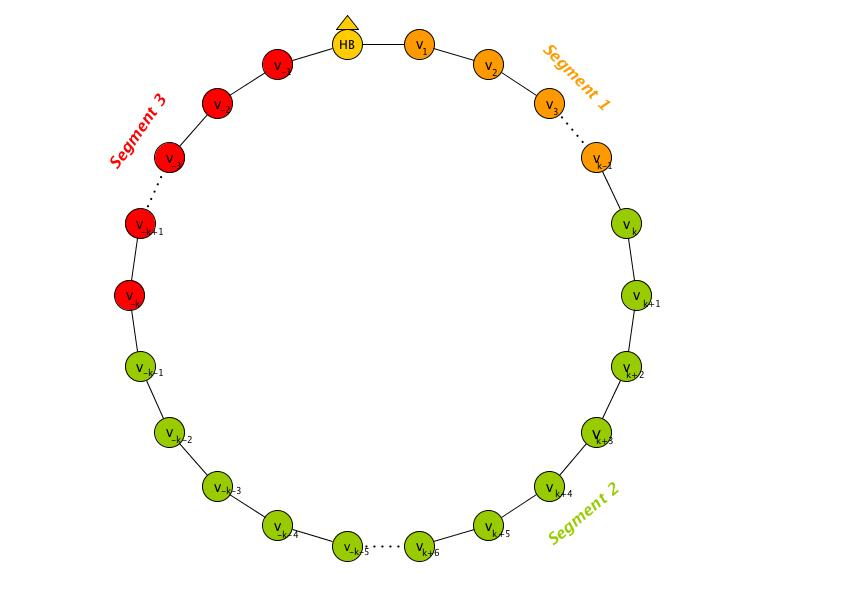
\includegraphics[width=0.6\textwidth]{figures/dloop_seg.jpg}
  \caption{Dividing the double loop into three segments.}\label{fig:dloop-seg}
\end{figure}



\begin{itemize}

\item  {\em Segment 1} contains nodes $v_1, \ldots v_{k-1}$.  If the \bv is in this segment, the size of the safe area is $1\leq |S_{area}| \leq k-1$.
%:  $1\leq i <k$
\item  {\em Segment 2} contains nodes $v_k, \ldots v_{n-k-1}$.   If the \bv is in this segment, the size of the safe area is $k\leq |S_{area}| \leq n-k-1$.
%: $k\leq i <n-k$
\item  {\em  Segment 3}  contains nodes $v_{n-k}, \ldots v_{n-1}$.   If the \bv is in this segment, the size of the safe area is $n-k\leq |S_{area}| \leq n-1$.
%: $n-k\leq i \leq n-1$
\end{itemize}

We will see that complexity changes depending on the  location of the black virus relative to the segment. 

The number of agents required to disinfect the double loop chordal ring $C$ is the same regardless of the strategy employed, whereas the number of moves varies depending on the deployment method.
 




\begin{theorem}\label{theo:agents}
Regardless of deployment strategy and chord length, a maximum of 12 agents are employed  in any double loop $C_n(1,k)$ for the black virus disinfection protocol.
\end{theorem}
\begin{proof}
The number of agents required is determined by the location of the original black virus, regardless of the deployment strategy.
\begin{itemize} 
\item
When the $BV$ is located at any node in  {\em Segment 1}, we would obtain  the worst complexity in terms of $CA$ and $SA$ since activating the \bv will create three more \bvs at $x_{1}$, $x_{k}$, and $ x_{-k}$. $LEA$ then  moves to $x_{0}$ and deploys seven  $SA$s to occupy $x_{2},x_{k-1},x_{k+1},x_{2k},x_{-k+1},x_{-k-1}$ and $x_{2k}$. The total number of agents employed is then 12:  $4$ $CA$s, $7$  $SA$s and one $LEA$. Thus, in this case,  $Spread(C)=4$ and $Size(C)=12$.   
 
\item If $BV$ is found in  {\em  Segment 2 },
%, $Spread(C)=3$, $Size(C)=6$.   
activating the original \bv would create two more \bvs at $x_{1}$ and $ x_{k}$ because $x_{-k}$ is guarded by a $SH$. $SH$ then moves to $x_{-k+1}$  and $LEA$ moves to $x_{0}$. $LEA$ then deploys $4$  $SA$s to occupy $x_{2},x_{k-1},x_{k+1}$ and $x_{2k}$. The total number of agents employed is then 9: $3$ $CA$s, $4$  $SA$s, $1$ $SH$ and $LEA$. Thus, in this case,  $Spread(C)=3$ and $Size(C)=9$.
 
\item If $BV$ is found in  {\em Segment 3}, there are two possible scenarios:

\begin{itemize}
\item 
%, $Spread(C)=2$, $Size(C)=4$.  \\
When $n-k \leq i < n-1$:\\ %$Spread(C)=2$, $Size(C)=4$, $Move(C)\leq7$.  \\ 
This segment is part of what is called  the {\it Danger area} ($D_{area}$).
% Since our protocol is monotone, the explored nodes should be protected from getting recontamination; therefore, more $SH$(s) are deployed.  
If the $BV$ is located at any node in this segment, activating the original \bv would create only one \bv at $x_{1}$, while $x_{-k}$ and $x_{k}$ are guarded by $SH$s. Subsequently, in addition to the $SH$ at $x_{-k+1}$, the $SH$ at $x_{k+1}$ and $LEA$ at $x_{0}$, the $LEA$ deploys $1$  $SA$ to occupy $x_{2}$. The total number of agents employed is then 6: $2$ $CA$s, $1$  $SA$, $2$ $SH$ and one $LEA$. Thus, in this case,  $Spread(C)=2$ and $Size(C)=6$.


\item When $i=n-1$, 
%$Spread(C)=1$, $Size(C)=4$.  \\ 
no more \bvs are created  since all neighbouring nodes of the \bv  are guarded by $SH$s and $LEA$. There are then no $SA$s to be deployed and all the moves are done in the first phase. The total number of agents employed is then 5: $1$ $CA$, $3$ $SH$s and one $LEA$. Thus, in this case,  $Spread(C)=.1$ and $Size(C)=5$.

\end{itemize}
\end{itemize}
\end{proof}




For the deployment phase we propose  two types of strategies: non-local and local. 
In   non-local strategies, $LEA$ calculates the shortest path to reach the various targets and gives each agent the information about the corresponding path. 
In local strategies, each $SA$ decides the next node locally, based on the indication of the destination target.
 


\subsection{Move-Optimal Deployment}



In this section we describe  a non-local approach where $SA$s follow paths set up by their leader $LEA$ who has full  topological knowledge. 
Once the \bv is triggered,  $LEA$, knowing the topology and the location of the black viruses, computes  the best route to each target and gives the information to the corresponding $SA$s.
Because of the simple structure of the chordal ring, we can calculate the exact length of the shortest paths to reach the target and verify experimentally that they are indeed optimal.

In this section we describe the path to be followed by each agent
%
%Essentially, once the \bv is triggered,  $LEA$ computes a breadth-first partial spanning tree of the chordal ring, excluding the contaminated nodes, to determine the shortest route to each target and passes the information to a $SA$  agent for each of them.
%To  describe the strategy and calculate its  complexity, 
for  the simpler case of   shortly-chorded double loops,  and  then for the    case of general double loops. 
 Before we describe these two situations  we will  identify  some special  constant size paths that can be used to reach all targets in both situations. The special path to reach node  $x_i$ from $x_0$ is denoted by $\sigma_i$.
Depending on the chord structure,  it may be possible to devise shorter paths in some cases. A detailed analysis of all possible situations is carried out in the next two sections.
 
 
\begin{center}
  \begin{tabular}{|c|c|}
 \hline
 Target $x_i$ & Special Path $\sigma_i$\\
 \hline
  $x_{k-1}$ &  $x_{0}\xrightarrow {-1}x_{-1}\xrightarrow {+k}x_{k-1}$\\
  $x_2$ & $x_{0} \xrightarrow {-1} x_{-1} \xrightarrow {+k} x_{k-1} \xrightarrow {+k} x_{2k-1} \xrightarrow {+1} x_{2k}  \xrightarrow {+1} x_{2k+1} \xrightarrow {+1} x_{2k+2} \xrightarrow {-k} x_{k+2} \xrightarrow {-k} x_{2}$\\
$x_{2k}$ &   $ x_{0} \xrightarrow {-1} x_{-1} \xrightarrow {+k} x_{k-1} \xrightarrow {+k} x_{2k-1} \xrightarrow {+1}  x_{2k}$\\
 $x_{k+1}$ & $ x_{0} \xrightarrow {-1} x_{-1} \xrightarrow {+k} x_{k-1} \xrightarrow {+k} x_{2k-1}
 \xrightarrow {+1}  x_{2k}\xrightarrow {+1} x_{2k+1} \xrightarrow {-k} x_{k+1}$\\
 $x_{-k-1}$ & $ x_{0} \xrightarrow {-1} x_{-1} \xrightarrow {-k} x_{-k-1}$\\
$x_{-k+1}$ & $ x_{0} \xrightarrow {-1} x_{-1} \xrightarrow {-k} x_{-k-1} \xrightarrow {-k} x_{-2k-1} \xrightarrow {+1} x_{-2k} \xrightarrow {+1} x_{-2k+1} \xrightarrow {+k} x_{-k+1}$\\
 $x_{-2k}$  & $x_{0} \xrightarrow {-1} x_{-1} \xrightarrow {-k} x_{-k-1} \xrightarrow {-k} x_{-2k-1} \xrightarrow {+1} x_{-2k}$\\
 \hline
 \end{tabular}
 \end{center}
 
 
\subsubsection {Shortly-chorded Double Loops}
\label{sec:shortly}

A shortly-chorded  double loop is a double loop where the size is significantly bigger than the length of the largest chord, that is:
  $k << n$. 
  All results of this section hold for $n > 4k$.
  % $C\{1,5\}$ and $n=100$.



After triggering the original $BV$ ($x_{0}$) the neighbouring nodes are in one of two states: guarded or contaminated.
Node $x_{-1}$ is guarded by $LEA$. Depending on the size of the {\it safe area}, nodes $x_{1}$, $x_{k}$ and $x_{-k}$ could be in either state.
As mentioned earlier, the \bv could be located in one of three segments.
\begin{comment}
\\ Here we have two scenarios: when $\left\vert{S_{area}}\right\vert \ge k$ and when $\left\vert{S_{area}}\right\vert< k$.

When $\left\vert{S_{area}}\right\vert \ge k$, $LEA$ has to deploy agents to the neighbours of the new two black viruses $\cal BV$=$\{x_1,x_k\}$  in order to clear them while $x_{-1}$ and $x_{-k}$ are already guarded by $LEA$ and $SH$.


Node  $x_{1}$ has two unoccupied neighbours N$_{un}$($x_{1}$)=\{$x_{2}$,$x_{k+1}$\} while $x_{1-k}$ is guarded by $SH$ that has moved from its previous location $x_{-k}$. Node $x_{k}$ has three unoccupied neighbours N$_{un}$($x_{k}$)=\{$x_{k-1}$,$x_{k+1}$,$x_{2k}$\}.  
Node $x_{k+1}$ is a common neighbour of $x_1$ and $x_k$.
Thus, we have that ${\cal T} = \{x_{2},x_{k-1},x_{k+1},x_{2k}\}$.
\end{comment}

 For some of the targets it is easy to identify the shortest path from $x_0$. For example,   $x_{k-1}$  cannot be reached directly but  it can  be reached in two moves from $x_0$  through node $x_{-1}$ (i.e.,  following the special path $\sigma_{k-1}$). For other targets  it is harder to determine whether $\sigma_i$ represents the best alternative.

%
We now  consider the different routes to each target in  four different  cases depending on the location of the {\it black virus} where $\pi[x_0,x_{i}] $ denotes a path to reach target $x_i$ from $x_0$. 

% Let $\pi[x_0,x_{i}] $ denote a path to reach target $x_i$. 

\begin{itemize}
\item {\bf Case 1}: Consider the case where the \bv is in the second segment of the chordal ring, that is, when $k\leq |S_{area}| <n-k$. In this case, triggering the original \bv creates two more {\it black viruses}: $x_{1}$ and $x_{k}$, and thus $\cal T$=$\{x_{2},x_{k-1},x_{k+1},x_{2k}\}$.
\begin{itemize}

\item  $x_{k-1}$:  Node  $x_{k-1}$ is reached through $\sigma_{k-1}$, which is clearly  the shortest path.

\item $x_{2}$: Since for   $k=3$ we know that $x_2 =  x_{k-1}$, we  consider $k>3$.\\
Depending on the length of $k$,  $x_{2}$  could be reached  optimally  in different ways (note that  all of them are actually shorter than  the special  path $\sigma_2$ identified earlier):\\


 \begin{itemize} 
 \item If  $k = 4$ and $x_{k-1}=x_3$,  the shortest path is the following: %the target is reached in 3 moves by :
$$ \pi[x_0,x_2] =   \pi_{1} =   x_{0}\xrightarrow {-1}x_{-1} \xrightarrow {+k}x_{k-1}=x_3\xrightarrow {-1}x_{2}$$
\item If   $k > 4$, taking advantage of the fact that $x_{-k}$ is known to be safe: 
%the target is reached in 4 moves as follows:
$$ \pi[x_0,x_2] =   \pi_{2}  =   x_{0}\xrightarrow {-k}x_{-k} \xrightarrow {+1}x_{1-k}\xrightarrow {+1}x_{2-k}\xrightarrow {+k}x_{2}$$
%\item If $k = 3$ %the target reached in two moves:
%$$   \sigma_{2}  =  x_{0}\xrightarrow {-1}x_{-1} \xrightarrow {+k}x_{2}$$
\end{itemize}


\item $x_{2k}$:    Node  $x_{2k}$ is reached through $\sigma_{2k}$.
% 
%$$\sigma_{2k} = x_{0} \xrightarrow {-1} x_{-1} \xrightarrow {+k} x_{k-1} \xrightarrow {+k} x_{2k-1} \xrightarrow {+1}  x_{2k}$$


\item$x_{k+1}$: 
If $ k >4$,    $x_{k+1}$ is reached through $\sigma_{k+1}$. 
Otherwise, it is reached faster  through:
$$ \pi[x_0,x_{k+1}] =    \pi_{3} =   x_{0}\xrightarrow {-1}x_{-1} \xrightarrow {+k}x_{k-1}=x_3 \xrightarrow {-1}x_{2}\xrightarrow {+k}x_{k+2}\xrightarrow {-1}x_{k+1}$$

%\item Otherwise, it is reached through  $\sigma_{k+1}$
%$$ \pi[x_0,x_{k+1}] =     \sigma_{k+1} =   x_{0} \xrightarrow {-1} x_{-1} \xrightarrow {+k} x_{k-1} \xrightarrow {+k} x_{2k-1}
% \xrightarrow {+1}  x_{2k}\xrightarrow {+1} x_{2k+1} \xrightarrow {-k} x_{k+1}$$
%\end{itemize}

\end{itemize}

 \item {\bf Case 2}: When the \bv is in the third   segment excluding the last node before the homebase
 (i.e.,   $n-k\leq |S_{area}| <n-1$), only  one \bv is generated ($x_1$) since the rest of the neighbours have been explored and guarded. Thus,
$\cal T$=$\{x_2,x_{k+1}\}$.
\begin{itemize}
\item $x_2$: 
 If  $k \leq4$,  $x_2$ is reached using $\pi_1$, otherwise  it is reached using $\pi_2$ \\
\item $x_{k+1}$ is reached in one move  from node $x_{k}$ because $x_{k}$ contains a $SH$ agent, which received a copy of the original {\it black virus}.  
\end{itemize}
\item  {\bf Case 3}: We have a special case in which the \bv is located  on the last node before the homebase. In this case, all neighbours are guarded and no more \bvs are created. The surrounding phase is no longer needed.

\item {\bf Case 4}:  When the \bv is in the first  segment  (i.e., $\left\vert{S_{area}}\right\vert < k$) 
 we have to  consider the nodes that might be contaminated  if they do not belong to the  area already protected by shadows.
In fact, when $\left\vert{S_{area}}\right\vert < k$, $LEA$ has to deploy agents to the neighbours of the three new black viruses $\cal BV$=$\{x_1,x_k,x_{-k}\}$ while $x_{-1}$ is being guarded by $LEA$ and no $SH$ has been deployed.


Node  $x_{-k}$ has three unguarded neighbours, N$_{un}$($x_{-k}$)$=\{x_{-k-1}$,$x_{-k+1}$,$x_{-2k}\}$.
Thus, ${\cal T} = \{x_{2},x_{k-1},x_{k+1},x_{2k},x_{-k-1},x_{-k+1},x_{-2k},\}$.


We have:
\begin{itemize}
\item Nodes $x_{k-1}$ and $x_{2k} $ are reached through paths $\sigma_{k-1}$ and $\sigma_{2k}$.
\item $x_{k+1}$ is reached through $\pi_3$ or $\sigma_{k+1}$ as   explained in {\bf Case 1}.


\item $x_{-k-1}$ is reached through path  $ \sigma_{-k-1}$.
 %is reached in two moves: \\
%$$  \sigma_{-k-1} =    x_{0} \xrightarrow {-1} x_{-1} \xrightarrow {-k} x_{-k-1}$$

\item \noindent  $x_{-2k}$ is reached through path $ \sigma_{-2k}$.  % is reached in  4 moves: 
 
%$$  \sigma_{-2k} = x_{0} \xrightarrow {-1} x_{-1} \xrightarrow {-k} x_{-k-1} \xrightarrow {-k} x_{-2k-1} \xrightarrow {+1} x_{-2k}$$

\item \noindent  $x_{-k+1}$ is reached through path $ \sigma_{-k-1}$.
% 
%$$\sigma_{-k+1} = x_{0} \xrightarrow {-1} x_{-1} \xrightarrow {-k} x_{-k-1} \xrightarrow {-k} x_{-2k-1} \xrightarrow {+1} x_{-2k} \xrightarrow {+1} x_{-2k+1} \xrightarrow {+k} x_{-k+1}$$ 

\item  $x_{2}$: In this case, node $x_{-k}$ is a \bv and any path that passes through it to reach $x_2$ should be avoided.
\begin{itemize}
\item if $k < 8$ , the path to reach $x_2$ is:
$$ \pi[x_0,x_{2}] =    \pi_{4} = x_{0} \xrightarrow {-1} x_{-1} \xrightarrow {+k} x_{k-1} \xrightarrow {-1} x_{k-2} \xrightarrow {-1},... \xrightarrow {-1} x_{2}$$
\begin{comment}
or
$$ \pi[x_0,x_{2}] = x_{0} \xrightarrow {-1} x_{-1} \xrightarrow {-1} x_{-2} \xrightarrow {-1} x_{-3} \xrightarrow {-1},... \xrightarrow {-1} x_{-k+2} \xrightarrow {+k} x_{2}$$
Actually both routes give the same number of moves.
\end{comment}
\item otherwise, (i.e. $k \ge 8$), $x_2$ is reached through $ \sigma_{2}$.
%
%$$ \sigma_{2} = x_{0} \xrightarrow {-1} x_{-1} \xrightarrow {+k} x_{k-1} \xrightarrow {+k} x_{2k-1} \xrightarrow {+1} x_{2k}  \xrightarrow {+1} x_{2k+1} \xrightarrow {+1} x_{2k+2} \xrightarrow {-k} x_{k+2} \xrightarrow {-k} x_{2}$$
%
\end{itemize}
\end{itemize}
\end{itemize}


%Note that  the deployment of agents in the shortly-chorded rings is always done following a standard %paths  to reach any of the targets.  
The following  theorems   summarize the number of moves:
%%%%%%%%%%%%%%%%%%%%%%%%%%%%%%%%%%%%%%
\begin{comment}
\begin{center}
  \begin{tabular}{|c|c|}
 \hline
 Destination & number of moves \\
 &\\
 \hline
$x_2$ & $\leq 8$ when $\left\vert{S_{area}}\right\vert < k$  \\   
&\\
& $\leq 4$ when $\left\vert{S_{area}}\right\vert \ge k$  \\   
&\\
\hline
 $x_{k-1}$ & $ 2$\\
 &\\
 \hline
 $x_{k+1}$ & $\leq 6$  \\ 
 &\\
 \hline
 $x_{2k}$ & $4$  \\ 
& \\
\hline
$x_{-k-1}$ & $2$  \\ 
 &\\
 \hline
$x_{-2k}$ & $4$  \\  %I don't have cases minimize the # of moves like the case of $x_{2k}$
 &\\
 \hline
$x_{-k+1}$ & $6$  \\ 
 &\\
 \hline
\end{tabular} 
 \end{center}


%%%%%%%%%%%%%%%%%%%%%%%%%%%%%%
\begin{center}
\begin{tabular}{|l|lr|lr|}\hline
\multirow{2}{1 in}{Destination} &
\multicolumn{2}{c|}{Number of moves}
\\
& $\left\vert{S_{area}}\right\vert < k$ & $\left\vert{S_{area}}\right\vert \ge k$ \\\hline\hline
$x_2$       & $\leq8$ & $\leq 4$  \\\hline
$x_{k-1}$    & $2$   & $2$     \\\hline
$x_{k+1}$ & $\leq 6$   & $\leq 6$         \\\hline
$x_{2k}$            & $4$   & $4$        \\\hline

$x_{-k-1}$    & $2$   & -     \\\hline
$x_{-2k}$ & $4$   & -        \\\hline
$x_{-k+1}$            & $6$   & $1$        \\\hline
$x_1$       & $1$ & $1$  \\\hline
$x_k$       & $1$ & $1$  \\\hline
$x_{-k}$       & $1$ & -  \\\hline
{\bf Total}     & $\leq 35$   & $\leq19$ \\\hline
\end{tabular}
\captionof{table}{Move-optimal complexity  in shortly-chorded double loop.}
\end{center}

\end{comment}



%The optimal  routes direction have to be decided according to the number of nodes $n$ and the %distance separating nodes   $x_k$ and $x_{-k}$ (i.e. $n-(2k$+1) )
 
%In order to do that, we divide the chordal ring into windows consist of $k+1$ nodes starting %from   $x_{0}$ as   follows.\\
%\begin {center}
%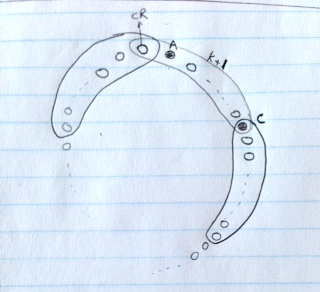
\includegraphics [scale=0.50] {windows.jpg}
%\end {center}

%% I have three windows, when n-(2k+1)=k-1, then +k and-k are delimiters of the third %%window.the more the difference decreases, the more overlapping the third window is with the %%other two windows., here we have another case to be handled in term of routing.

%If the partitioning results in two windows between the k$^{th}$ nodes of $x_{0}$,i.e if %$n-(2k+1) \leq 2k $ ($n\leq 4k+1$),  then the routing direction is better to be the counter %clockwise, otherwise, the clockwise direction is better route in terms of the number of moves.






 



 \begin{theorem}
In any shortly-chorded  double loop   $C_n(1,k)$,  if $\left\vert{S_{area}}\right\vert \ge k$, 
the number of moves to complete the  {\em Surrounding  and Eliminating} phase is a maximum of $20$.
%4+2+6+4+2 the last 2 is for sending two casualties +1 for SA to guard x_{-k+1}
%\leq 18 because of x_2 and x_{k+1} can be fewer than 4
\end{theorem}
%%%%%%%%%%%%%%%%%%
 \begin{proof}

 The first move is made by $LEA$ to move to $x_0$. Then, by construction, we know that:
\begin{itemize}
\item $k\leq |S_{area}| <n-k$
\begin{itemize}

\item Node $x_{k-1}$ is reached in two moves through path $\sigma_{k-1}$

\item 
In the case of node $x_{2}$ we have three possibilities:  if $k > 4$,  the target is reached in four moves;  if $k = 4$,  the target is reached in three moves; if $k = 3$, $x_2$ coincides with $x_{k-1}$ and the target is reached in two moves.  The maximum amount of moves is thus four.


\item $x_{2k}$ is reached in four moves through path $\sigma_{2k}$

\item $x_{k+1}$ follows the same route as $x_{2k}$ in the clockwise direction with the addition of two moves,
or from $x_{2}$  with the addition of two more moves. The algorithm selects the minimum. The maximum number of moves in this case is then six.

\end{itemize}

 \item $n-k\leq |S_{area}| <n-1$\\
In this case, one \bv is generated ($x_1$) since the neighbouring nodes are guarded. Thus,
$\cal T$=$\{x_2,x_{k+1}\}$.
\begin{itemize}
\item $x_2$ is reached in maximum four moves, corresponding to path $\pi_2$
\item $x_{k+1}$ is reached in one move since the $SH$ at node $x_{k}$ received a copy of the original {\it black virus}, and $SH$s always make one move in the clockwise direction when they receive a {\it black virus} in order to be part of the surrounding team.
\end{itemize}

\end{itemize}

%In any shortly-chorded double loop chordal ring, if $\left\vert{S_{area}}\right\vert \ge k$ and in the existence of two $BV$s, the maximum number of moves required to reach all targets is at most six.
Since all of the agents are sent at the same time they will arrive at their destinations within six time units.
After waiting six time units, the $LEA$  will send two agents to clear the two \bvs, thus performing two more moves.
\end{proof}

\begin{theorem} 
In any shortly-chorded  double loop   $C_n(1,k)$, if $\left\vert{S_{area}}\right\vert < k$,
the number of moves to complete the  {\em Surrounding  and Eliminating} phase is a maximum of $36$.
\end{theorem}

 \begin{proof}
One move is made by $LEA$ to move to $x_0$. Then, by construction,  if  $\left\vert{S_{area}}\right\vert < k$, we know that: node  $x_{k+1}$ is reached within six moves through $\sigma_{k+1}$ or $\pi_3$; 
node  $x_{k-1}$ is reached within two moves through $\sigma_{k-1}$;
node  $x_{2k}$ is reached within four moves through $\sigma_{2k}$;
node   $x_{-k-1}$ is reached within two moves through $\sigma_{-k-1}$;
node    $x_{-2k}$ is reached within four moves through $\sigma_{-2k}$;
  $x_{-k+1}$ is  reached through $x_{-2k}$ with the addition of two more moves through path $\sigma_{-k+1}$, which means a maximum of six moves;
node $x_{2}$. In this case $x_2$ is reached through $\sigma_{2}$ or $\pi_4$ and the number of moves would be a maximum of eight. After all the agents arrive at their destinations, three more moves are needed to clear the black viruses. 

\end{proof}


 %------------------------------------------------------------------------------ 
\subsubsection{General Double Loop}
\label{sec:general}


In this section, we handle double loop chordal rings in general $C_n(1,k)$, where  $2 < k  < \lfloor\frac{n}{2}\rfloor$. 
Finding the exact optimal number of moves in this  case is much more complicated and difficulties arise because, depending on the length of the chords and the number of nodes,  it may be more convenient to wrap around the ring in order to reach certain targets.

In order to describe the {\em Surrounding and Eliminating} process we use the same notations and cases. In other words, we have two cases: when $\left\vert{S_{area}}\right\vert \ge k$ and when $\left\vert{S_{area}}\right\vert < k$. Therefore, the set of targets ${\cal T}$ is  $=\{x_{2},x_{k-1},x_{k+1},x_{2k},x_{-2k},x_{-k+1},x_{-k-1}\}$,  $=\{x_{2},x_{k-1},x_{k+1},x_{2k}\}$, $=\{x_{2},x_{k+1}\}$ or $\emptyset$ . The only difference between this section and the previous one is in the {\it deployment} part of the algorithm since, as mentioned above, we have more possibilities in the general structure of the double loop. 


\medbreak
\noindent {\bf Case   $\left\vert{S_{area}}\right\vert \ge k$.}  Let us first consider the case in which $\left\vert{S_{area}}\right\vert \ge k$. 
  For some targets, the path to be followed is the same as the one employed for shortly chorded rings. This is the case for $x_{k-1}$ and $x_2$. Node  $x_{k-1}$  is reached through $\sigma_{k-1}$.  If  $k = 4$,  node $x_{2}$  is reached through $  \pi_{1} $; otherwise, it is reached through $\pi_2$.


In the following discussion we will refer to the special paths  $\sigma_i$  identified in the  previous section  and compare them to other possible routes in order to find the best one.

 In order to find the best routes to reach nodes $x_{k+1}$ and $x_{2k}$, we divide the ring into "windows" of size ($k+1$) starting from $x_0$ in both directions, and consider different cases depending on the number of windows covering the ring.

\begin{enumerate}

\item  $\lceil {n \over k} \rceil >  4$.

 Intuitively,   $n$  is big enough for us to consider this a Shortly-chorded double loop and we follow the same paths indicated in the previous section to reach the target.


\item  $\lceil {n \over k} \rceil=  4$.

\begin{figure}[H]
  \centering  
  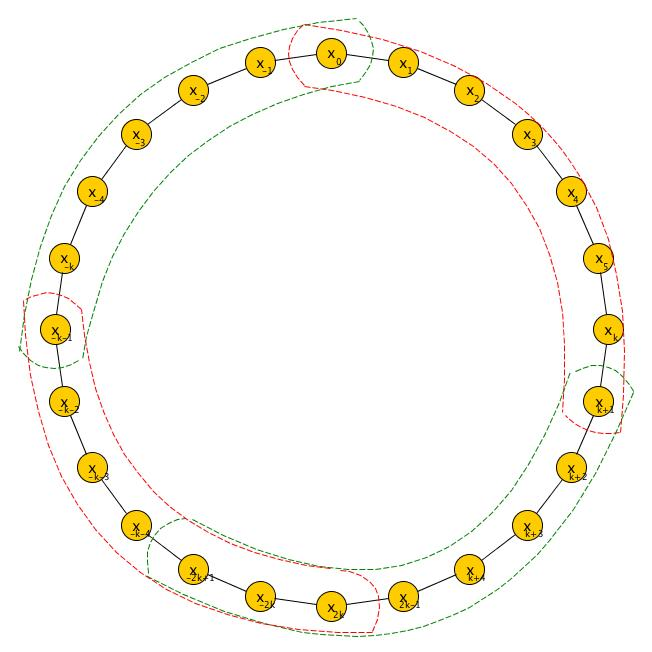
\includegraphics[width=0.5\textwidth]{figures/dloop_window2.jpg}
  \caption{Dividing the outer ring into 4 windows of size $k+1$.}\label{fig:dloop-window}
\end{figure}

 
 In this case it might be  more efficient to ``wrap-around" the chordal ring to reach  both  $x_{k+1}$ and $x_{2k}$.
%In this case  we have 4 windows  with a non empty intersection. To reach $x_{2k}$,  we take the %counter clockwise direction. 
 %Note that   the number of elements in that  intersection  (i.e $4k-n+1$)  is either  1 , 2 or 3.
%      ( $4k-n$ the distance between $x_{-2k}$ and $x_{2k}$ in the intersection)
      
  \begin{itemize}    
\item $x_{2k}$. \\
To reach target $x_{2k}$ we distinguish between different situations depending on the relationship
 between $n$ and $k$: \\
--- If $n=4k$
 $$ \pi[x_0,x_{2k}]  = x_{0} \xrightarrow {-k} x_{-k} \xrightarrow {-k} x_{-2k} \xrightarrow {-1} x_{2k}$$

---  If   $k < {2\over7}n-1$

$$ \pi[x_0,x_{2k}] = \min \{ \pi_5, \sigma_{2k}\}$$
where

$$ \pi_5 = x_{0} \xrightarrow {-k} x_{-k} \xrightarrow {-k} x_{-2k} \xrightarrow {+1} x_{-2k+1}\xrightarrow {+1} ... \xrightarrow {+1} x_{2k}$$
and $ \sigma_{2k}$ is the special path we referred to in shortly-chorded loops.
$$ \sigma_{2k}=   x_{0} \xrightarrow {-1} x_{-1} \xrightarrow {+k} x_{k-1} \xrightarrow {+k} x_{2k-1}
 \xrightarrow {+1}  x_{2k}$$
%in this case  the number of moves is $4k-n+2$ ( $4k-n$ the distance between $x_{-2k}$ and %$x_{2k}$ in the intersection). \\
%However, if $\left\vert{\pi_1}\right\vert > 4$, then the agent take the standard path  $\pi_s$.\\ \\

--- If    $k \leq {2\over7}n-1$
$$ \pi[x_0,x_{2k}] = \min \{ \pi_6,  \sigma_{2k}\}$$
 
 where 
 
$$\pi_6 = x_{0} \xrightarrow {-k} x_{-k} \xrightarrow {-1} x_{-k-1} \xrightarrow {-1} x_{-k-2}\xrightarrow {-1} ... \xrightarrow {-1} x_{2k}$$
%However, if $\left\vert{\pi_2}\right\vert > 4$, then the agent take $\pi_s$.\\
%and the number of moves is $n-3k+1$ ($n-3k$ is the distance between $x_{-k}$ and $x_{2k}$ %\\ \\

 

 \item $x_{k+1}$    \\
--- If $n=4k$
$$ \pi[x_0,x_{k+1}]  = x_{0} \xrightarrow {-k} x_{-k} \xrightarrow {-k} x_{-2k} \xrightarrow {-k} x_{k+1}$$
% To reach $x_{k+1}$,  %%$x_{-2k}$is closer to $x_{k+1}$, so it is better to 
%take the route:\\
---Else 
$$ \pi[x_0,x_{k+1}] = \min \{ \pi_7,  \sigma_{k+1}\}$$

where
 
$$ \pi_7 = x_{0} \xrightarrow {-k} x_{-k} \xrightarrow {-k} x_{-2k} \xrightarrow {-1} x_{-2k-1}\xrightarrow {-1} ... \xrightarrow {-1} x_{k+1}$$
%However, if $\left\vert{\pi_1}\right\vert > \left\vert{\pi_s}\right\vert$, then the agent take $\pi_s$.\\
%and the number of moves will be $n-3k+1$.
% n-2k-k-1 the difference between the two nodes +2 moves to reach $x_{-2k}$

and $ \sigma_{k+1}$ is the path to reach $x_{k+1}$ in shortly-chorded loops.

$$  \sigma_{k+1} =   x_{0} \xrightarrow {-1} x_{-1} \xrightarrow {+k} x_{k-1} \xrightarrow {+k} x_{2k-1}
 \xrightarrow {+1}  x_{2k}\xrightarrow {+1} x_{2k+1} \xrightarrow {-k} x_{k+1}$$


\end{itemize}

\item  $\lceil {n \over k} \rceil<  4$ 

\begin{itemize}
 \item $x_{k+1}$.
In this case, in addition to $\sigma_{k+1}$, there are three other  possibilities and we have:
$$ \pi[x_0,x_{k+1}] = \min \{\sigma_{k+1}, \pi_8,\pi_9,\pi_{10}\}$$

\begin{itemize}
\item  (* when the $+k^{th}$ neighbour of $x_{k+1}$  is between $x_{-1}$ and $x_{-k}$, it might be advantageous to move to $x_{-1}$ first *)
   $$ \pi_8 = x_{0} \xrightarrow {-1} x_{-1} \xrightarrow {-1} x_{-2} \xrightarrow {-1} ... \xrightarrow {-1} x_{2k+1}\xrightarrow {-k} x_{k+1}$$ % number of moves $n-2k$
\item (*  if instead  $x_{-k}$  is closer to $x_{2k+1}$ , then  it might be better to move to first $x_{-k}$ *)
$$ \pi_9 = x_{0} \xrightarrow {-k} x_{-k} \xrightarrow {+1} x_{-k+1} \xrightarrow {+1} ... \xrightarrow {+1} x_{2k+1}\xrightarrow {-k} x_{k+1}$$ % number of moves $3k-n+3$
 \item (* finally, if $x_{-k}$  is closer to $x_{k+1}$ *)
$$ \pi_{10} = x_{0} \xrightarrow {-k} x_{-k} \xrightarrow {-1} x_{-k-1} \xrightarrow {-1} ... \xrightarrow {-1} x_{k+1}$$ % number of moves $n-2k$ 
\end{itemize}

 
\item $x_{2k}$. Target $x_{2k}$ resides   between $x_{-1}$ and $x_{-k}$, so we first have to determine which of them is closer.  We have: 

$$ \pi[x_{11},x_{k+1}] = \min \{   \sigma_{2k}, \pi_{11}, \pi_{12}\}$$

where

$$\pi_{11} = x_{0} \xrightarrow {-1} x_{-1} \xrightarrow {-1} x_{-2} \xrightarrow {-1} ... \xrightarrow {-1} x_{2k}$$ % number of moves $n-2k$

$$\pi_{12} =  x_{0} \xrightarrow {-k} x_{-k} \xrightarrow {+1} x_{-k+1} \xrightarrow {+1} ... \xrightarrow {+1} x_{2k}$$ % number of moves $3k-n+1$
 
% and $ \sigma_{k+1}$ is the standard path to reach $x_{k+1}$.


\end{itemize}

\end{enumerate}




 
\noindent {\bf Case    $\left\vert{S_{area}}\right\vert < k$.} 
Consider now the case in which
  $\left\vert{S_{area}}\right\vert < k$. In this case: ${\cal T}$$=\{x_{2}$, $x_{k-1}$, $x_{k+1}$, $x_{2k}$, $x_{-2k}$, $x_{-k+1}$, $x_{-k-1}\}$.   Notice here that in all cases,  any route that passes through $x_{-k}$ should be avoided because $x_{-k}$ is now a {\it black virus}. 

\begin{itemize}

  \item  Nodes $x_{k-1}$, $x_{-2k}$, $x_{-k+1}$, and $x_{-k-1}$ are reached through the paths $\sigma_{k-1}$, $\sigma_{-2k}$, $\sigma_{-k+1}$ and $\sigma_{-k-1}$ respectively.
 



\item To find the best routes to reach nodes $x_2$, $x_{k+1}$ and $x_{2k}$, we also use the concept of "windows"  mentioned earlier.
\begin{enumerate}


\item  $\lceil {n \over k} \rceil >  4$ \\
This case is the same as the shortly-chorded chordal ring structure and uses the methodology described in the previous section.

\item  $\lceil {n \over k} \rceil=  4$ 
 
%In this case  we have 4 windows  with a non empty intersection. To reach $x_{2k}$,  we take the %counter clockwise direction. 
 %Note that   the number of elements in that  intersection  (i.e $4k-n+1$)  is either  1 , 2 or 3.
%      ( $4k-n$ the distance between $x_{-2k}$ and $x_{2k}$ in the intersection)
      
  \begin{itemize}    
\item $x_{2k}$.  (* The only option   besides the route $ \sigma_{2k}$ is  $\pi_{13}$ described below, which should be taken only   if $n=4k+1$. *)
 $$\pi_{13} = x_{0} \xrightarrow {-1} x_{-1} \xrightarrow {-k} x_{-k-1} \xrightarrow {-k} x_{2k}$$
 
% $$ \pi[x_0,x_{2k}] = \min \{   \sigma_{2k}, \pi_{13}\}$$

 \item $x_{k+1}$ 
  $$ \pi[x_0,x_{k+1}] = \min \{   \sigma_{k+1}, \pi_{14}\}$$
  where
$$\pi_{14} = x_{0} \xrightarrow {-1} x_{-1} \xrightarrow {-k} x_{-k-1} \xrightarrow {-k} x_{-2k-1} \xrightarrow {-1} x_{-2k-2}\xrightarrow {-1} ... \xrightarrow {-1} x_{k+1}$$

 
%and the number of moves will be $n-3k+1$.
% n-2k-k-1 the difference between the two nodes +2 moves to reach $x_{-2k}$





%\begin {center}
%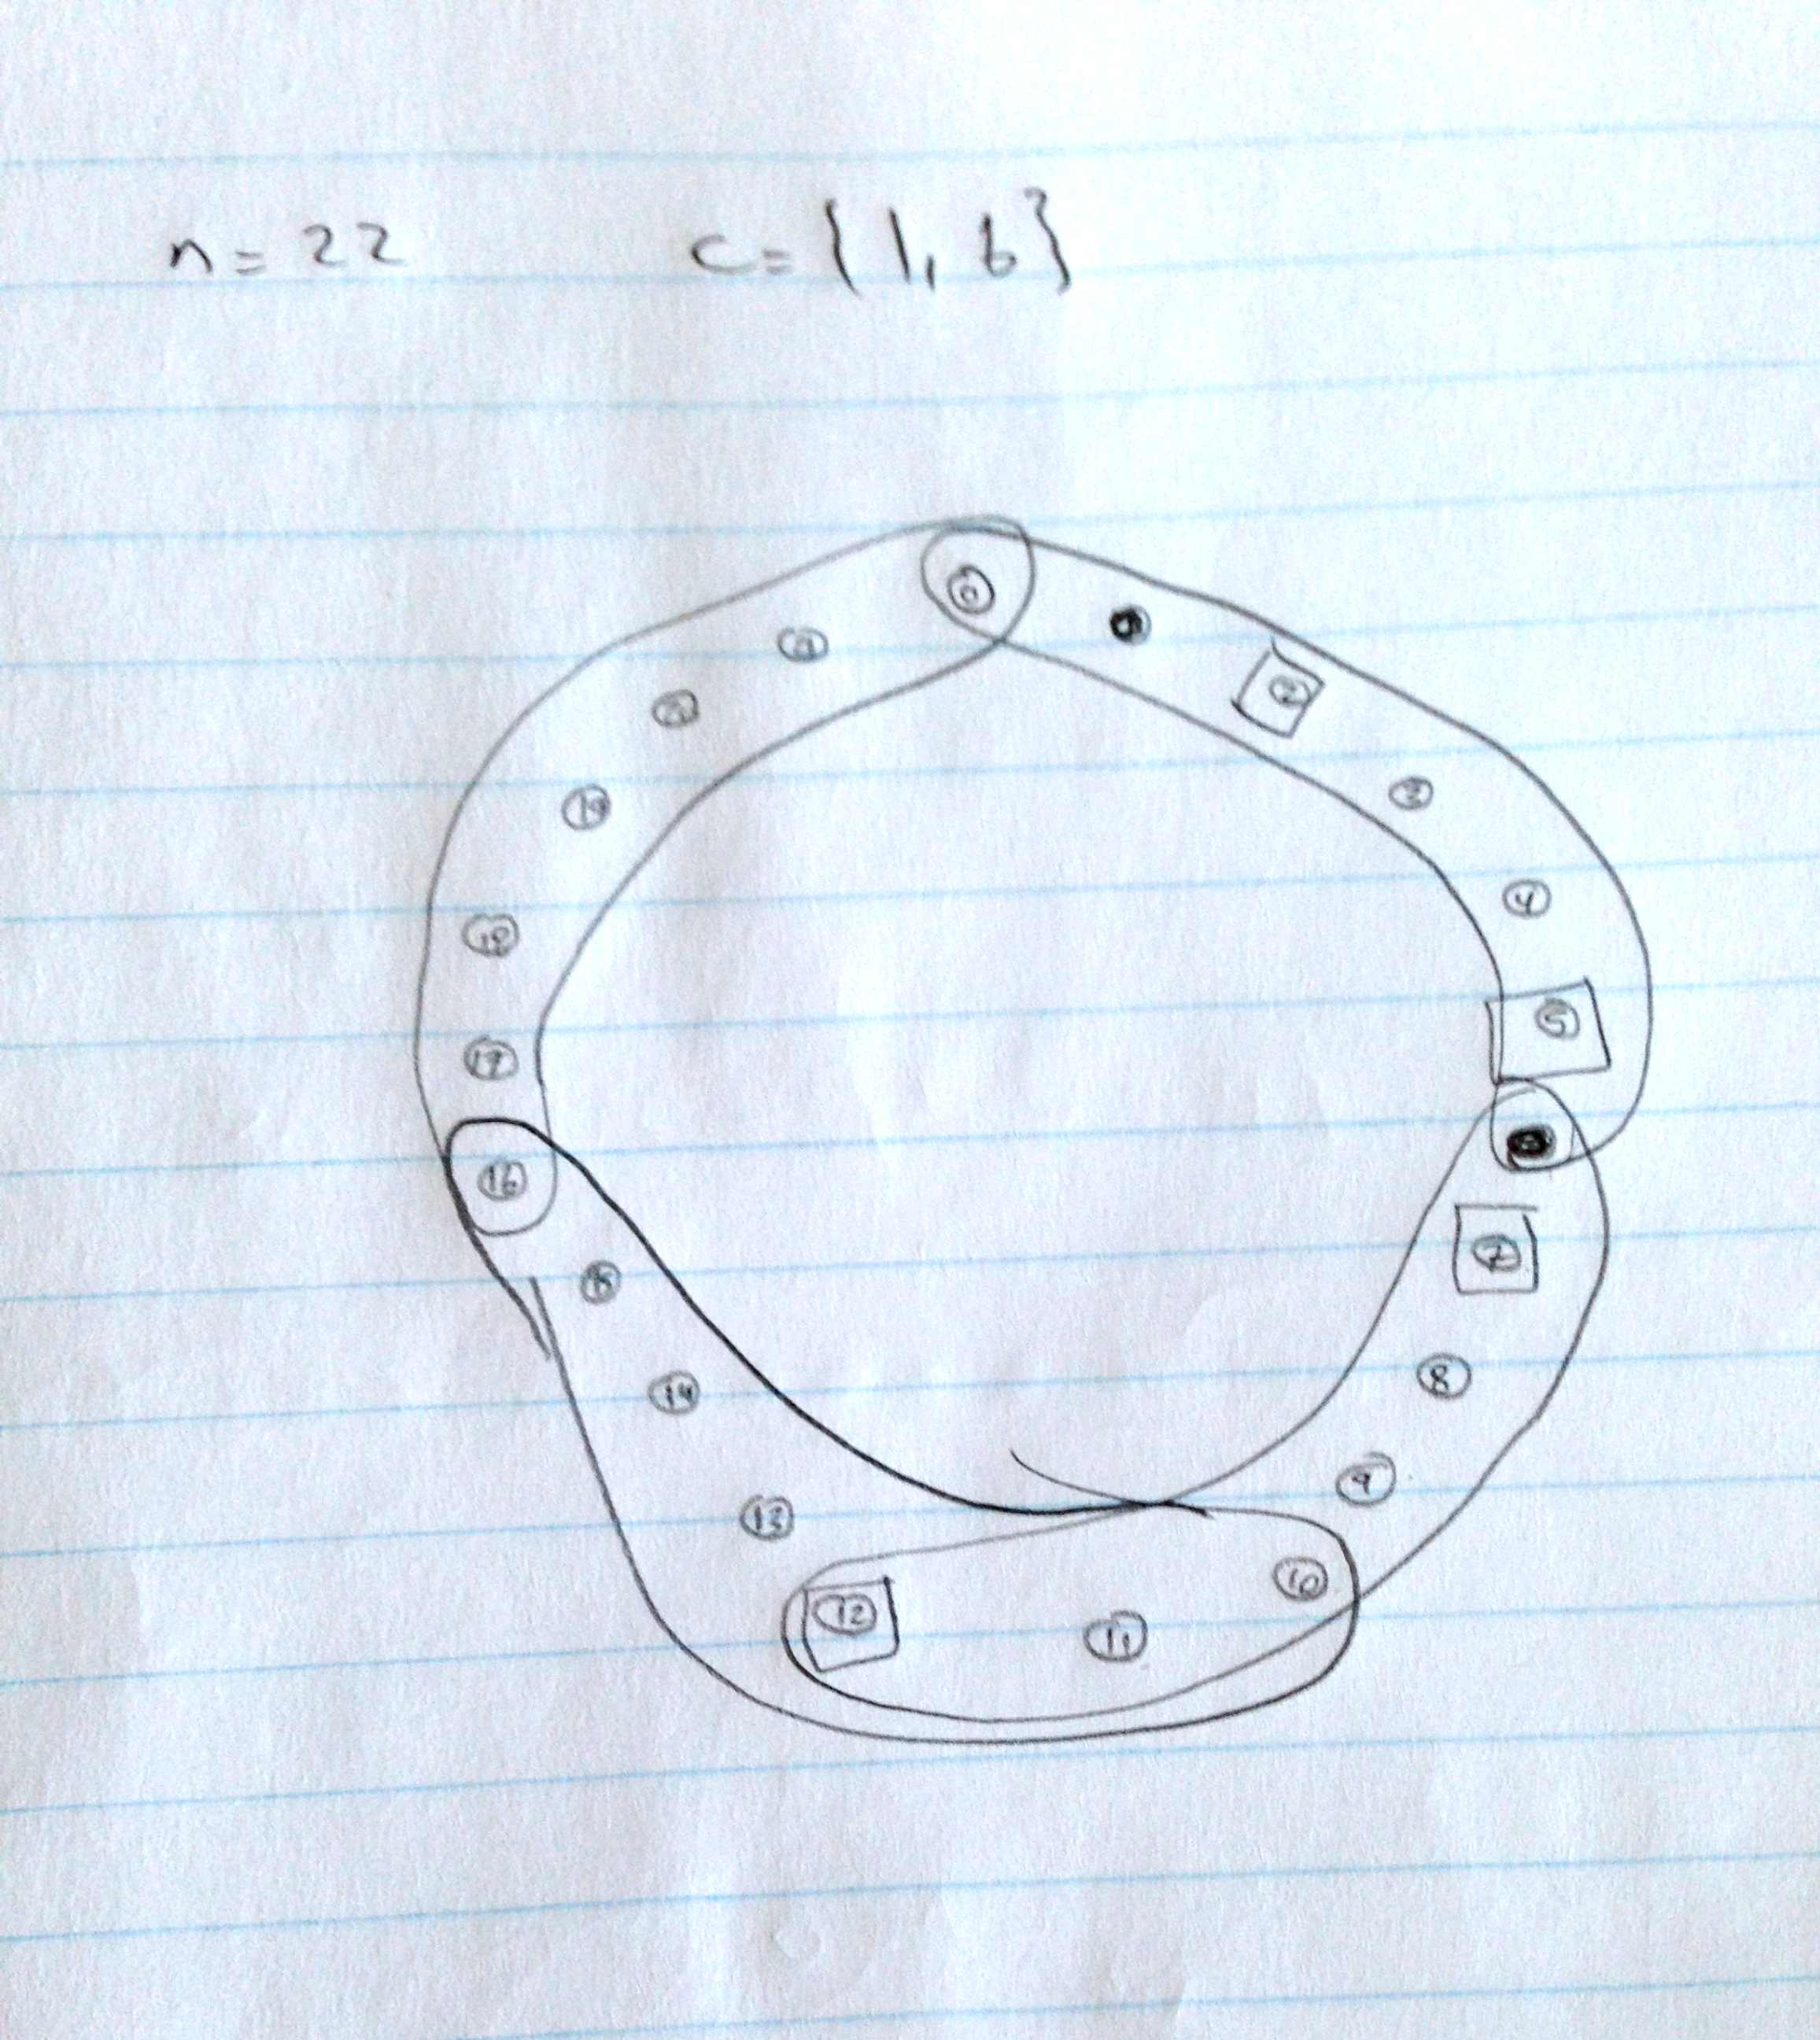
\includegraphics [scale=0.10] {intersection.jpg}
%\end {center}

\item $x_{2}$:
 $$ \pi[x_0,x_{2}] = \min \{   \sigma_{2},\pi_{4},\pi_{15}\}$$
where

 
$$\pi_{15} = x_{0} \xrightarrow {-1} x_{-1} \xrightarrow {-k} x_{-k-1} \xrightarrow {-k}x_{-2k-1} \xrightarrow {-k} x_{-3k-1}\xrightarrow {-1} ... \xrightarrow {-1} x_{2}$$
Notice here that if $n=4k+1$, the agent cannot take   route $\pi_{15}$ 
 because node $x_{-3k-1} =x_{k}$. 

\end{itemize}

 \item  $\lceil {n \over k} \rceil<  4$ \\
\begin{itemize}


 \item $x_{k+1}$  
In this case, in addition to the path $\sigma_{k+1}$, there are the following possibilities leading to:

  $$ \pi[x_0,x_{k+1}] = \min \{   \sigma_{k+1}, \pi_{16}, \pi_{17}\}$$

\begin{itemize}
\item  (* The $+k^{th}$ neighbour of $x_{k+1}$  is between $x_{-1}$ and $x_{-k}$, so 
if $x_{-1}$ is closer then: *)

   $$\pi_{16} = x_{0} \xrightarrow {-1} x_{-1} \xrightarrow {-1} x_{-2} \xrightarrow {-1} ... \xrightarrow {-1} x_{2k+1}\xrightarrow {-k} x_{k+1}$$ % number of moves $n-2k$

 \item (*  $x_{-k}$  is closer to $x_{k+1}$  *)
$$\pi_{17} = x_{0} \xrightarrow {-1} x_{-1} \xrightarrow {-k} x_{-k-1} \xrightarrow {-1} ... \xrightarrow {-1} x_{k+1}$$ 
% number of moves $n-2k$ 
\end{itemize}


 \item $x_{2k}$
   $$ \pi[x_0,x_{2k}] = \min \{   \sigma_{2k}, \pi_{18}\}$$

 
$$ \pi_{18} = x_{0} \xrightarrow {-1} x_{-1} \xrightarrow {-1} x_{-2} \xrightarrow {-1} ... \xrightarrow {-1} x_{2k}$$ % number of moves $n-2k$
 
 
 \item $x_{2}$
 
   $$ \pi[x_0,x_{2}] = \min \{   \sigma_{2},\pi_{4},\pi_{15}\}$$




\end{itemize}

\end{enumerate}
\end{itemize}

%{\bf Paola: to be explained.} From the   results of Sections \ref{shortly} and \ref{general},
% we found that the results coincide {\bf ???}; therfore, we combine them in the following table, which summarizes the number of moves required in the surrounding and eliminating phase for any double loop chordal ring.
 

%
%
%\begin{theorem}
%In any double loop   $C_n(1,k)$,  if $\left\vert{S_{area}}\right\vert \ge k$,  $spread(G)=3$ and $size(G) \leq 6$.
%\end{theorem}
%%%%%%%%%%%%%%%%%%%
% \begin{proof}
%   If $\left\vert{S_{area}}\right\vert \ge k$, and a $BV$ is triggered, it affects 2 of its 4 neighbours.
%
% Let $x_0$ be the original black virus, node $x_{-1}$ is clearly protected by LEA, $x_{1} $ and $x_{k}$ are surely affected, on the other hand 
%After triggering and clearing the $BV$, one agent is dead, and since we get two more $BV$s, the number of casualties is 3. \\
%The newly created $BV$s are $x_{1}$, and $x_{k}$. To clear them, their neighbours have to be guarded. 
%Node  $x_{1}$ has two unoccupied neighbours, N$_{un}(x_{1})=\{x_{2},x_{k+1}\}$, and two guarded neighbour, N$_{ex}(x_{1})=\{x_{-k+1},x_{0}\}$.
%Node $x_{k}$ has three unoccupied neighbours, N$_{un}(x_{k})=\{x_{k-1},x_{k+1},x_{2k}\}$, and one guarded node, N$_{ex}(x_{k})=\{x_{0}\}$.
%Node $x_{k+1}$, and of course $x_{0}$ are common neighbours of $x_1$ and $x_k$ and already guarded by $LEA$ and $SH$.
%Thus, we have that the set of targets ${\cal T} = \{x_{2},x_{k-1},x_{k+1},x_{2k}\}$, so the number of agents needed to guard the neighbours of $BV$s is at most 6, $size(G) \leq 6$; notice that it could be less if we have more common neighbours. Therefore, the total number of agents needed to decontaminate the whole topology is at most 9, $spread(G)=3$ and $size(G) \leq 6$. 
% 
%\end{proof}
%
%
%\begin{theorem}
%In any double loop $C_n(1,k)$,  if $\left\vert{S_{area}}\right\vert < k$,  $spread(G)=4$ and $size(G) \leq 8$.
%\end{theorem}
% \begin{proof}
% 
%Let   $\frac{n}{4} <k  < n$.  If $\left\vert{S_{area}}\right\vert < k$, and a $BV$ is triggered, it affects 3 of its 4 neighbours (i.e.$x_{-k}$  is not guarded). Therefore, in addition to the four agents we need to guard ( $x_{2}$,$x_{k+1}$,$x_{k-1}$,$x_{2k}$) , we need three  more to cover the neighbours of $x_{-k}$, which are $x_{-k-1}$, $x_{-k+1}$ and $x_{-2k}$. Notice that $x_{-k+1}$ is a mutual neighbour between $x_{1}$ and $x_{-k}$. In other words, the total number of agents needed to surround $BV$s in the worst case is maximum 8 including $LEA$. 
%\\ Since we have 3 $BV$s in this case, then the number of casualties is 4.
%\end{proof}

We have seen that the case of the shortly-chorded ring is simpler to study, however, the number of moves employed to reach the targets is the same in both cases and leads to the same complexity. 
 
 \begin{theorem}
In any double loop   $C_n(1,k)$,  if $\left\vert{S_{area}}\right\vert \ge k$,  
the number of moves to complete the  {\em Surrounding  and Eliminating} phase is a maximum of $20$.
\end{theorem}
 \begin{proof}
In any double loop chordal ring, if $\left\vert{S_{area}}\right\vert \ge k$, the maximum number of moves required to reach all targets is $20$.
One move is done by $LEA$ to reach $x_0$.
By construction, whether  $\lceil {n \over k} \rceil >  4$ or  $\lceil {n \over k} \rceil \leq  4$, the nodes are reached as follows: 
node $x_{2k}$ is reached within four moves; node $x_{k+1}$ is reached within six moves;
node $x_{k-1}$ is reached within two moves and node $x_{2}$ is reached within four moves.
 

Since we always compare the resulting routes $\pi_z$, where $z \in \mathbb{Z}$,  to the special ones in the shortly-chorded loops $\sigma_i$, none of $\pi_z$ would be greater than the corresponding $\sigma_i$. 

After all the agents have arrived at their destinations, one move is done by the $SH$ and two moves are needed to send $CA$s.
\end{proof}

\begin{theorem}
In any double loop  $C_n(1,k)$,  if $\left\vert{S_{area}}\right\vert < k$, 
the number of moves to complete the Surrounding and Eliminating phase is a maximum of 36.
\end{theorem}

 \begin{proof}
At the beginning of the second phase, one move is made by the $LEA$ to move to $x_0$. Then, whether  $\lceil {n \over k} \rceil >  4$ or  $\lceil {n \over k} \rceil \leq  4$, the nodes are reached as follows: 
 node $x_{2k}$ is reached within four moves; node $x_{k+1}$ is reached within six moves and node $x_{k-1}$ is reached within two moves. Node $x_{2}$ is reached by taking any route except the one that passes through $x_{-k}$, and the number of moves would be a maximum of eight. Node $x_{-k-1}$ is reached within four moves; node $x_{-k+1}$ is reached within six moves and node $x_{-2k}$ is reached within four moves.


Since we always compare the resulting routes $\pi_z$, where $z \in \mathbb{Z}$,  to the ones  in the shortly-chorded loops $\sigma_i$, none of $\pi_z$ would be greater than the corresponding $\sigma_i$. 

After all agents arrive at their destinations, only three moves are needed to disinfect the topology.
\end{proof}
 The following table summarizes the number of moves required in the {\em Surrounding and Eliminating} phase in any double loop chordal ring.


%%%%%%%%%%%%%%%%%%%%%%%%%%%%%
\begin{comment}
\begin{center}
  \begin{tabular}{|c|c|}
 \hline
 Destination & number of moves \\
 &\\
 \hline
$x_2$ & $\leq 8$ when $\left\vert{S_{area}}\right\vert < k$  \\   
&\\
& $\leq 4$ when $\left\vert{S_{area}}\right\vert \ge k$  \\   
&\\
\hline
 $x_{k-1}$ & $ 2$\\
 &\\
 \hline
 $x_{k+1}$ & $\leq 6$  \\ 
 &\\
 \hline
 $x_{2k}$ & $\leq4$  \\ 
& \\
\hline
$x_{-k-1}$ & $2$  \\ 
 &\\
 \hline
$x_{-2k}$ & $4$  \\  %I don't have cases minimize the # of moves like the case of $x_{2k}$
 &\\
 \hline
$x_{-k+1}$ & $6$  \\ 
 &\\
 \hline
\end{tabular} 
 \end{center}
\end{comment}
%%%%%%%%%%%%%%%%%%%%%%%%%%%%%%%%%%


\begin{center}
\begin{tabular}{|l|lr|lr|}\hline
\multirow{2}{1 in}{Destination} &
\multicolumn{2}{c|}{Number of moves}
\\
& $\left\vert{S_{area}}\right\vert < k$ & $\left\vert{S_{area}}\right\vert \ge k$ \\\hline\hline
$x_0$       & $1$ & $1$  \\\hline
$x_2$       & $\leq8$ & $\leq 4$  \\\hline
$x_{k-1}$    & $2$   & $2$     \\\hline
$x_{k+1}$ & $\leq 6$   & $\leq 6$         \\\hline
$x_{2k}$            & $\leq 4$   & $\leq 4$        \\\hline

$x_{-k-1}$    & $2$   & -     \\\hline
$x_{-2k}$ & $4$   & -        \\\hline
$x_{-k+1}$            & $6$   & $1$        \\\hline
$x_1$       & $1$ & $1$  \\\hline
$x_k$       & $1$ & $1$  \\\hline
$x_{-k}$       & $1$ & -  \\\hline
{\bf Total}     & $\leq 36$   & $\leq 20$ \\\hline
\end{tabular}
\captionof{table}{Move complexity  in double loops.}
\end{center}



%%%%%%%%%%%%%%%%%%%%%
\begin{theorem}\label{correctnes_mo}
The  algorithm  following  the move-optimal deployment strategy successfully disinfects a double loop chordal ring from \bvs in a monotone synchronous way.
\end{theorem}
\begin{proof}
Destroying a \bv is done only if it moves to a guarded node. Therefore, in this phase, agents surround all the neighbouring nodes  and then $LEA$ activates them so they move to neighbouring nodes. As previously mentioned, the crucial part is the routing, and in this strategy (Move-optimal), $LEA$ is responsible for directing agents to their destinations. Since $LEA$ has the topological knowledge, it correctly calculates the targets and sets up the paths for $SA$s.
\end{proof}
 %------------------------------------------------------------------------------ 
\subsubsection{On Optimality and Other Observations}\label{local-opt}
 

 We ran a simulation to construct a partial  {\it Breadth-First Search} tree rooted in $x_0$ 
in double loops  with "missing nodes" corresponding to the black viruses triggered in the various scenarios. The spanning tree was constructed until all the targets appeared as leaves. In this type of spanning tree, any path from $x_0$ to a target leaf is the shortest path from $x_0$  to that destination.

We exhaustively tested all the different scenarios depending on the location of the black virus. Note that the size of the chordal ring influences the length of the shortest path for each scenario: 
 1) Shortly-chorded double loops when $|S_{area}|<k$, 2) Shortly-chorded double loops when $|S_{area}|\ge k$, 3) General double loops where $n\leq4k$ when $|S_{area}|<k$ and 4) General double loops where $n\leq4k$ when $|S_{area}|\ge k$.
In all the scenarios above we verified that the paths indicated are indeed the shortest paths.

\medbreak

As a final note,  if all agents have full knowledge of the topology and of the targets,   the aforementioned approach can be transformed into a {\em local strategy} where agents decide their next step without referring back to the $LEA$. In each step, an agent could locally construct a breadth first search tree in order to find the shortest path to their target. They could then pick the neighbour that satisfies the following conditions:  not a $BV$,  not a predecessor and on the shortest path.
After all the agents reach their destinations, $LEA$ triggers the $BV$s by sending the cleaning agents. This strategy is optimal and local, yet it is compute-intensive. It requires the same number of agents and moves as the aforementioned move-optimal algorithm.



\subsection{Simple Greedy Deployment}
 
In the previous section, the proposed algorithm is controlled by the $LEA$ who has a map for the entire topology. Once he finds the original $BV$, he decides the best routes and sends agents through them. The only job the agents have to do is following the paths set by the leader and stored in their memories. In this section we introduce some strategies that rely completely on local decisions. 
In other words, instead of carrying the whole path, the agent calculates its next move for each step until it reaches its target. 

Consider  the following simple local Greedy strategy: an agent at some node $source$, having to reach a node $dest$, chooses as a  next link the one that takes it closest to $dest$. The distance is calculated on the outside ring.
Note that, in a double loop {\em without viruses}, this simple greedy strategy  would correspond to optimal routing  
 between any pair of nodes. 



Let $link(source, dest)$ be the next link to be taken from node $source$ to eventually reach node $dest$.
It  is easy to see that the   greedy strategy described above corresponds to the following local choice:  %%{\bf Please, check all my indices, I did it in a hurry and you know I easily introduce %%mistakes }

\[
 link(x_i,x_j)  =    \left\{ \begin{array}{ll}
          \mbox{ if  $(i-j)\leq (n-j+1)$ }  &  go-clockwise:  \\
          \tab    \tab  \mbox  { if  $ (j-i)  <  k  $}   & \mbox  {take-link  +1}\\
                    \tab    \tab  \mbox  {otherwise}   & \mbox   {take-link  $+k $}\\

          \ \\
          \mbox{ if  $(i-j)> (n-j+1)$ }  &  go-counter-clockwise:  \\
          \tab   \tab \mbox  {if  $ (n-j+i)  <  k  $} &  \mbox  {take-link  -1}\\
                    \tab    \tab  \mbox  {otherwise}   & \mbox   {take-link  $-k $}\\
                          \end{array} \right. \] 
        
\noindent In order to occupy the target nodes, we have the following optimal paths where the BV has been underlined:

\begin{center}
  \begin{tabular}{|c|c|}
 \hline
 Target & Greedy path  \\
 &\\
 \hline
$x_2$ &$[x_0,$ \underline{$x_1$},$x_2]$\\
&\\
\hline
 $x_{k-1}$ & $[x_0,$ \underline{$x_k$},$x_{k-1}]$\\
 &\\
 \hline
 $x_{k+1}$ & $[x_0,$ \underline{$x_k$},$x_{k+1}]$\\
 &\\
 \hline
 $x_{2k}$ & $[x_0,$ \underline{$x_k$},$x_{2k}]$\\
 &\\
\hline
\end{tabular}
\captionof{table}{Greedy path without {\it black viruses.}}
 
 \end{center}
  
  
In the presence of $BV$s to be avoided, the greedy strategy will give correct but non-optimal routing. 
The advantage of this approach is that the surrounding 
agents do not carry a pre-determined path  and movement decisions are made locally.
 

 The greedy strategy can be described as follows. $dist(x,y)$ represents the shortest distance between nodes  $x$ and $y$ along the ring.
\begin{center}
\fbox{
\begin{minipage}{7.5cm}
{\sc Simple Greedy}
\begin{tabbing}
Depl\=oying agent $A$ arriving at $v$ from $y$ with destination $z$\\ \ \\

\> Let $FD =\{ N(v)- {\cal BV} - y \}$ be the set of possible destinations.\\
\> Agent $A$ moves to $w \in FD$ that minimizes $dist(w,z)$

\end{tabbing}
\end{minipage}
}
\end{center}
 
Note that the first step in any surrounding strategy is  always counter-clockwise, regardless of the destination, because both clockwise neighbours of $x_0$ are $BV$s. For example, an agent wants to reach $x_2$ from $x_0$ when $k>5$.  The agent would move to $x_{-1}$ and would continue to move counter-clockwise until reaching node $x_{-i}$ such that $i+3> -i+k-2$ ($2i>k-5$, $i =  \lceil{{ k-5} \over 2}\rceil$).
At this point the agent would take the clockwise chord $+k$ which gets it closer to $x_2$, and then would proceed counter-clockwise towards it by using chords -1. Notice that when $k\leq5$, $i$=1.

All the resulting greedy paths when  $\left\vert{S_{area}}\right\vert \ge k$ are outlined in the table below. For simplicity, we assume that $5<k<\lfloor {n \over 2} \rfloor$ and $k<<n$.

\begin{center}
  \begin{tabular}{|c|c|c|}
 \hline
 Target & Greedy path with $BV$s & Number of moves \\
 
 \hline
$x_2$ &$[x_0, x_{-1}, x_{-2},\ldots, x_{-i},x_{-i+k}, x_{-i+k-1},\ldots.... x_2]$ & \\
&$i =  \lceil{{ k-5} \over 2}\rceil$  & $k-1$ \\ 
\hline
 $x_{k-1}$ & $[x_0, x_{-1}, x_{k-1}]$ & $2$ \\

 \hline
 $x_{k+1}$ &  $[x_0, x_{-1}, x_{k-1}, x_{k-2}, x_{k-3},.... x_{k-i}, x_{2k-i}, x_{2k-i-1}, \ldots, x_{k+1}]$ &\\
    &  $i = \lceil{{ k-3} \over 2}\rceil$   & $k+1$ \\
 
 \hline
 $x_{2k}$ & $[x_0, x_{-1}, x_{k-1}, x_{2k-1},x_{2k}]$ & $4$ \\ %(if $ \lceil{n \over k}\rceil>4$ )\\
              %  & $[x_0, x_{-k}, x_{-2k},x_{-2k-1}....,x_{2k} $ (if $ \lceil{n \over k}\rceil \leq 4$)\\

\hline
\end{tabular} 
\captionof{table}{Greedy paths with \bvs when $\left\vert{S_{area}}\right\vert \ge k$ }\label{greedy-path}

 \end{center}
\begin{theorem}
In any double loop  $C_n(1,k)$,  if $\left\vert{S_{area}}\right\vert \geq  k$ and $k>5$, to surround and eliminate the {\it black viruses},
 the total number of moves performed by the Simple Greedy strategy is $\leq 2k+10$.
\end{theorem}
\begin{proof}
The first move in this phase is performed by $LEA$ in order to move from $x_{-1}$ to $x_0$, then the routing begins. When  $\left\vert{S_{area}}\right\vert \ge k$, after activating the original {\it black virus}, we might have two {\it black viruses}, one \bv or none depending on where the original \bv resides.
If we have two {\it black viruses}, ${\cal T}$$=\{x_{2},x_{k-1},x_{k+1},x_{2k}\}$, and the agents reach them as in table \ref{greedy-path} and the number of moves is obtained as follows: node $x_{2}$ is reached in $(k-1)$ moves; node $x_{k-1}$ is reached in two moves; node $x_{2k}$ is reached in four moves; node $x_{k+1}$ is reached in $(k+1)$ moves. The $SH$ at $x_{-k}$ makes one move to occupy $x_{-k+1}$, and $LEA$ sends two $CA$s in two moves to disinfect the whole topology.

\end{proof}

\noindent All the greedy paths when $\left\vert{S_{area}}\right\vert < k$ are outlined in the following table.

\begin{center}
  \begin{tabular}{|c|c|c|}
 \hline
 Target & Greedy path with $BV$s & Number of moves 
\\
 \hline
$x_2$ &$[x_0, x_{-1}, x_{-2},\ldots, x_{-i},x_{-i+k}, x_{-i+k-1},\ldots.... x_2]$ &\\
&$i =  \lceil{{ k-5} \over 2}\rceil$ & $k-1$ \\
\hline
 $x_{k-1}$ & $[x_0, x_{-1}, x_{k-1}]$ & $2$ \\

 \hline
 $x_{k+1}$ &  $[x_0, x_{-1}, x_{k-1}, x_{k-2}, x_{k-3},.... x_{k-i}, x_{2k-i}, x_{2k-i-1}, \ldots, x_{k+1}]$ &\\
    &  $i = \lceil{{ k-3} \over 2}\rceil$  & $k+1$ \\
 
 \hline
 $x_{2k}$ & $[x_0, x_{-1}, x_{k-1}, x_{2k-1},x_{2k}]$ & $4$ \\ %(if $ \lceil{n \over k}\rceil>4$ )\\
              

\hline

$x_{-k-1}$ &$[x_0, x_{-1}, x_{-k-1}]$ & $2$ \\

\hline
 $x_{-k+1}$ & $[x_0, x_{-1}, x_{-k-1}, x_{-k-2},.... x_{-k-i}, x_{-i}, x_{-i-1}, x_{-i-2}, \ldots, x_{-k+1}]$ &\\
  &  $i = \lceil{{ k-3} \over 2}\rceil$ & $k+1$ \\
 \hline
 $x_{-2k}$ &  $[x_0, x_{-1}, x_{-k-1}, x_{-2k-1},x_{-2k}]$ & $4$ \\

 

\hline
\end{tabular} 
\captionof{table}{Greedy paths with \bvs when $\left\vert{S_{area}}\right\vert < k$ }\label{greedy-path2}

 \end{center}

As mentioned above, the greedy algorithm does not produce  optimal paths.
For example, consider the case   $C_n\{1,6\}$  with  $ \lceil{n \over k}\rceil>4$.
To reach   $x_{2}$ using the   strategy  described in the previous section
 requires four moves while in the greedy strategy the agent  requires five moves.

 



\begin{theorem}
In any double loop  $C_n(1,k)$,  if $\left\vert{S_{area}}\right\vert < k$  and $k>5$, to surround and eliminate the {\it black viruses},
 the total number of moves performed by the Simple Greedy strategy is $3k+17$.
\end{theorem}
\begin{proof}
The first move in this phase is performed by $LEA$ to move from $x_{-1}$ to $x_0$, then the routing begins. When  $\left\vert{S_{area}}\right\vert < k$, after activating the original {\it black virus}, we  have three {\it black viruses}. Thus ${\cal T}$$=\{x_{2},x_{k-1},x_{k+1},x_{2k},x_{-k-1},x_{-k+1},x_{-2k}\}$ and the agents reach them as in table \ref{greedy-path2} as follows:
node $x_{2}$ is reached in $(k-1)$ moves;
node $x_{k-1}$ is reached in two moves;
node $x_{2k}$ is reached in four moves;
node $x_{k+1}$ is reached in $(k+1)$ moves;
node $x_{-k-1}$ is reached in two moves;
node $x_{-2k}$ is reached in four moves;
node $x_{-k+1}$ is reached in $(k+1)$ moves. The $LEA$ then sends three $CA$s in three moves to disinfect the whole topology.
\end{proof}
\begin{comment}
We now show that the Greedy algorithm is correct; i.e., that it   always lead the $SA$s to their targets in double loops regardless  of $k$.

\begin{theorem}\label{loop_free}
In any double loop chordal ring $C_n(1,k)$,  our simple Greedy strategy does the routing correctly with no infinite loops. 
\end{theorem}
\begin{proof}

The Greedy paths we indicated are loop free by construction.


Recalling our assumptions in our simple greedy strategy, we clearly stated that when an agent arrives at node $v$ from node $y$ to a target $z$, the agent checks the neighbours of its current residence and excludes  neighbours that are \bvs or  the node it just has come from, $y$. Since the agents have sense of directions, they would never return back to the nodes they just left. 
%The problem of going back to an already-visited node arises when as an agent goes greedily on the outer ring, it goes further from its destination; for example if the destination =$x_{2}$. So it is certain that one of its neighbours is closer to that destination from its current location; however, that neighbour is always $y$, the $\pm 1$ neighbour, so it never considers that neighbour as its next step. 


Assume by contradiction that our   greedy approach in double loop chordal rings is not loop-free and an agent would get stuck in an infinite loop by going back to an already-visited node. At any node $x_{i}$, an agent would have $N(x_{i})=\{x_{i\pm1}x_{i\pm k}\}$
Let us assume that we have $t=x_2$ and $k>5$. In order to reach that target, an agent moves from $x_0$ towards $x_{-1}$ since $x_{-1}$ is the closest safe neighbour to $x_{2}$.  At node $x_{-1}$, the agent would have $N(x_{-1})=\{x_{-2},x_{-k-1},x_{k-1}x_{0}\}$. Among those neighbours, $x_{-2}$ is the most suitable candidate to move to since $x_0$ is the node that the agent has just left. As this process carries on, from node $x_{-1}$ to  $x_{-2}$ and then $x_{-3}$ and so on, since each agent only would return back to an already-visited node if and only if that node is its neighbour through the chord $+ k$ that means that agent should passes through at least $k$ nodes which means that we need to reach node $x_{-k}$ in order to return back to an already-visited node and form a loop; however, node $x_{2}$ is directly connected to node $x_{-k-2}$ so there is no way an agent would keep moving until node $x_{-k}$. Similarly, we can prove the correctness of reach node $x_{k+1}$. 
Thus, we can see that before agents get stuck in infinite loops, they would reach their targets.
\end{proof}
\end{comment}



\subsection{Smart Greedy Deployment}
This algorithm is similar to the greedy algorithm except that this one takes the $k^{th}$ chords into consideration.
 


\begin{center}
\fbox{
\begin{minipage}{7.5cm}
{\sc Smart Greedy}
\begin{tabbing}
Depl\=oying agent $A$ arriving at $v$ from $y$ with destination $z$\\ \\
 Agent $A$ calculates $next$.\\

\tab Let $FD =\{ N(v)- {\cal BV} - y \}$ be the set of possible destinations.\\
\tab For each $v_i \in N(v)$\\

\tab\tab Let $d_i=dist(v_i,z)$ \\
\tab \tab If $d_i \ge k$  \\
\tab \tab $d_i= \lfloor{d_i \over k}\rfloor + (d_i \mod k)$ \\
 $next \in FD$ that has $v_i$ with the minimum $d_i$ \\
\tab If there is a tie between two or more of $N(v)$ \\
\tab \tab {\sc  tie-break}.\\

 Agent $A$ moves to $next$ 


\end{tabbing}
\end{minipage}
}
\end{center}
 
\begin{center}
\fbox{
\begin{minipage}{7.5cm}
{\sc tie-break}
\begin{tabbing}

\tab $v_i,v_j \in N(v)$ where $v_i ,v_j \notin BV$ and $dist(v_i,z)=dist(v_j,z)$\\
 Agent $A$ calculates $next$ \\
\tab Check $N(v_i)$ and $N(v_j)$\\

\tab\tab For each $u \in N(v_i)$ and $w \in N(v_j)$ where $u,w \notin N(v)$ --- are not predecessors\\

\tab\tab\tab Let $u_i=dist(v_i,z)$ and $w_j=dist(v_j,z)$ \\
\tab \tab\tab for each  $u_i$ or $w_j$ that is $ \ge k$  \\
\tab \tab\tab\tab change the distance to the value $ \lfloor{dist \over k}\rfloor + (dist \mod k)$ \\
\tab  $next$  $\in N(v)$ the has the neighbour with the minimum distance. 

\end{tabbing}
\end{minipage}
}
\end{center}

The smart greedy algorithm is local, yet it requires agents to do more calculations than the simple greedy algorithm. The complexity of this algorithm is not optimal. For example, to reach $x_{k+1}$ in a shortly-chorded double loop, the agent needs $>six$ moves.

In the smart greedy algorithm, we consider the longest chord which plays an important role in decreasing the distance between the two nodes. Therefore, if the $dist(x,y)\ge k$, there is one or more long chords between $x,y$ which minimizes the distance significantly. For example, if $dist(x,y)=10$ in $C_n(1,7)$, the actual distance is not $10$ but $4$ as we can see in the following equation:
$dist(x,y)= \lfloor{10 \over 7}\rfloor + (10 \mod 7) =4$.
Also, in this strategy, we attempted to resolve the situation in which two neighbours have the same distance to a target. If there is a tie, before the $SA$ chooses, it checks the neighbours and finds the minimum among them. If the tie persists, the $SA$ checks the neighbours of the neighbours until it breaks the tie. However, if the $SA$ finds two neighbours have a common neighbour that gives the minimum distance, it can pick any of them as in the case of reaching $x_{k+1}$ as we will see.


\noindent All the resulting smart greedy paths when  $\left\vert{S_{area}}\right\vert \ge k$ are outlined in the table below. For simplicity, we assume that $5<k<\lfloor {n \over 2} \rfloor$  and $k<<n$. 
\begin{center}
  \begin{tabular}{|c|c|c|}
 \hline
 Target & Smart Greedy path with $BV$s & Number of moves 
\\
 \hline
$x_2$ &$[x_0, x_{-k}, x_{-k}, x_{-k+1},x_{-k+2}, x_2]$ & $4$ \\

\hline
 $x_{k-1}$ & $[x_0, x_{-1}, x_{k-1}]$ & $2$\\

 \hline
 $x_{k+1}$ &  $[x_0, x_{-1}, x_{k-1}, x_{k-2}, .... x_{k-i}, x_{2k-i}, x_{2k-i-1}, \ldots, x_{k+1}]$ &\\
    &  $i = \lceil{{ k-3} \over 2}\rceil$  & $k+1$ \\  

 
 \hline
 $x_{2k}$ & $[x_0, x_{-1}, x_{k-1}, x_{2k-1},x_{2k}]$ & $4$ \\

\hline
\end{tabular} 
\captionof{table}{Smart greedy paths with \bvs when $\left\vert{S_{area}}\right\vert \ge k$ }\label{smart-path}

 \end{center}

\begin{theorem}
In any double loop  $C_n(1,k)$ where $\left\vert{S_{area}}\right\vert \geq  k$ and $k>5$, to surround and eliminate the {\it black viruses},
 the total number of moves performed by the Smart Greedy strategy is $\leq k+15$.
\end{theorem}
\begin{proof}
The first move in this phase is performed by $LEA$ to move from $x_{-1}$ to $x_0$, then the routing begins.
When  $\left\vert{S_{area}}\right\vert \ge k$, after activating the original {\it black virus}, we might have two {\it black viruses}, one \bv or none depending on where the original \bv resides.
If we have two {\it black viruses}, ${\cal T}$$=\{x_{2},x_{k-1},x_{k+1},x_{2k}\}$ and the agents reach them as in table \ref{smart-path} as follows:
node $x_{2}$ is reached in four moves; node $x_{k-1}$ is reached in two moves; node $x_{2k}$ is reached in four moves; node $x_{k+1}$ is reached in $(k+1)$ moves.
The $SH$ at $x_{-k}$ makes one move to occupy $x_{-k+1}$, and $LEA$ sends two $CA$s in two moves to disinfect the whole topology.
\end{proof}

\noindent  When $\left\vert{S_{area}}\right\vert < k$, all the resulting greedy paths are outlined in the table below.

\begin{center}
  \begin{tabular}{|c|c|c|}
 \hline
 Target & Smart Greedy path with $BV$s & Number of moves\\

 \hline
$x_2$ &$[x_0, x_{-1}, x_{-2},\ldots, x_{-i},x_{-i+k}, x_{-i+k-1},\ldots.... x_2]$ &\\
&$i =  \lceil{{ k-5} \over 2}\rceil$    & $k-1$\\
\hline
 $x_{k-1}$ & $[x_0, x_{-1}, x_{k-1}]$ & $2$ \\

 \hline
 $x_{k+1}$ &  $[x_0, x_{-1}, x_{k-1}, x_{k-2}, x_{k-3},.... x_{k-i}, x_{2k-i}, x_{2k-i-1}, \ldots, x_{k+1}]$ &\\
    &  $i = \lceil{{ k-3} \over 2}\rceil$  & $k+1$\\  
 
 \hline
 $x_{2k}$ & $[x_0, x_{-1}, x_{k-1}, x_{2k-1},x_{2k}]$ & $4$ \\ %(if $ \lceil{n \over k}\rceil>4$ )\\
              

\hline

$x_{-k-1}$ &$[x_0, x_{-1}, x_{-k-1}]$ & $2$ \\

\hline
 $x_{-k+1}$ & $[x_0, x_{-1}, x_{-k-1}, x_{-2k-1}, x_{-2k}, x_{-2k+1}, x_{-k+1}]$ & $6$ \\

 \hline
 $x_{-2k}$ &  $[x_0, x_{-1}, x_{-k-1}, x_{-2k-1},x_{-2k}]$ & $4$ \\

 

\hline
\end{tabular} 
\captionof{table}{Smart greedy paths with \bvs when $\left\vert{S_{area}}\right\vert < k$ }\label{smart-path2}

 \end{center}

%
%\begin{property}  
%The Smart Greedy algorithm is optimal in double loops with $BV$s only if $k \leq 5$ and $ \lceil{n \over k}\rceil>4$ .
%\end{property}  
%\begin{proof}  
%
%{\bf Not sure.}
%
%According to the results shown in the previous table, we can see that if $k \leq 5$, $ \lceil{n \over k}\rceil>4$ and $|S_{area}| \ge k$., we get the optimal number of moves which is at most 19.
%\begin{itemize}
%\item $x_{2}$ is reached in $\leq4$ moves as the following:
%$$x_{0} \xrightarrow {-1} x_{-1} \xrightarrow {+k} x_{k-1} \xrightarrow {-1} x_{k-2} \xrightarrow {-1} ... \xrightarrow {-1} x_{2}$$
%\item $x_{k-1}$ is reached in $2$ moves.
%$$x_{0} \xrightarrow {-1} x_{-1} \xrightarrow {+k} x_{k-1}$$
%\item $x_{2k}$ is reached in $4$ moves.
%$$x_{0} \xrightarrow {-1} x_{-1} \xrightarrow {+k} x_{k-1} \xrightarrow {+k} x_{2k-1} \xrightarrow {+1} x_{2k}$$
%\item $x_{k+1}$ is reached in $\leq6$ moves.
%$$x_{0} \xrightarrow {-1} x_{-1} \xrightarrow {+k} x_{k-1} \xrightarrow {+k} x_{2k-1} \xrightarrow {+1} x_{2k} \xrightarrow {+1} x_{2k+1} \xrightarrow {-k} x_{k+1}$$
%\end{itemize}
%The optimality holds when $|S_{area}| < k$.
%\end{proof}
 



\begin{theorem}
In any double loop  $C_n(1,k)$,  if $\left\vert{S_{area}}\right\vert < k$ and $k>5$, to surround and eliminate the {\it black viruses},
 the total number of moves performed by the Smart Greedy strategy is $2k+22$.
\end{theorem}
\begin{proof}
The first move in this phase is performed by $LEA$ to move from $x_{-1}$ to $x_0$, then the routing begins.
When  $\left\vert{S_{area}}\right\vert < k$, after activating the original {\it black virus}, we have three {\it black viruses}. Therefore,  ${\cal T}$$=\{x_{2},x_{k-1},x_{k+1},x_{2k},x_{-k-1},x_{-k+1},x_{-2k}\}$ and the agents reach them as in \ref {smart-path2} as follows:
node $x_{2}$ is reached in $(k-1)$ moves; node $x_{k-1}$ is reached in two moves; node $x_{2k}$ is reached in four moves; node $x_{k+1}$ is reached in $(k+1)$ moves; node $x_{-k-1}$ is reached in two moves; node $x_{-2k}$ is reached in four moves; node $x_{-k+1}$ is reached in six moves.
The $LEA$ then sends three $CA$s in three moves to disinfect the whole topology.
\end{proof}

\begin{comment}

\begin{theorem}\label{loop_free2}
In any double loop chordal ring $C_n(1,k)$,  our smart Greedy strategy does the routing correctly with no infinite loops. 
\end{theorem}
\begin{proof}
Follows the same proof as \ref{loop_free}.
\end{proof}

\end{comment}
\section{Conclusion}  
In this chapter we investigated the two phases required to disinfect a double loop chordal ring from {\it black viruses}.  
The first phase is common to all deployment strategies. In fact, as we will see throughout this thesis, this phase uses the same technique for all chordal rings. On the other hand, the second phase of double loop chordal rings has different possible routing strategies: move-optimal, simple greedy and smart greedy. The whole algorithm correctly disinfects any double loop chordal ring, regardless of the routing strategy.

% This is not really a proof.
%\begin{theorem}
%The  disinfection algorithm  successfully disinfect a double loop chordal ring from \bvs in a monotone synchronous way following either deployment strategy (Move-optimal, Greedy, Smart Greedy). 
%\end{theorem}
%\begin{proof}
%Due to the structure of the double loop chordal ring, $C_n(1,k)$ where $2<k<\lfloor\frac{n}{2}\rfloor$, the algorithm consisting of the two phases  correctly does the disinfection in a monotone synchronous way. Since we have two additional chords connected to each node in the ring, it is quiet easy to manage the monotonicity as we showed in the first phase, see \ref{monotone_ph1}. In the second phase, regardless of the deployment strategy and due to the synchronicity of our execution, all $SA$s will be at their targets surrounding the \bvs within a specific amount of time, then $LEA$ will clear all the \bvs at once. For each deployment strategy, we discussed its correctness, see \ref{correctnes_mo}, \ref{loop_free}, \ref{loop_free2}.
%
%\end{proof}
In the following tables we combine the complexities of the two phases for the three routing strategies proposed for disinfecting any double loop chordal ring.

\begin{comment}
OK, Still to be discussed.
%%%%%%%%%%%%%%%%%%%%%%%%%%%%
\begin{theorem}
In any double loop  $C_n(1,k)$, {\bf we need to explain where those
$3k+30$ moves mentioned at the beginning  come from.}
\end{theorem}
May be it's better to add a section or change section comparison to something else so I can be able to add the total of the two phases.
%%%%%%%%%%%%%%%%%%%%%%%%%%%%%%

In this section, we will summarize and compare the results we obtained from the aforementioned two sections.

{\bf If this is only for shorted chorded we have to move it.}
 
{\bf To discuss.}




Summary of complexities ....

From Theorem  \ref{theo:agents}: Agents:

Number of Moves:


{\bf What we said in the table at the beginning   has to be explained:}
 
 Move-Optimal , 4, 8 (isn't it 12 ?), $3k+30$   
\end{comment}





\begin{center}
\scalebox{0.9}{
\begin{tabular}{|l|l|lr|lr|lr|}\hline
\multirow{2}{1.2 in}{$BV$ at node $v_i$} &
\multirow{2}{1.2 in}{Phase 1} & 

\multicolumn{2}{c|}{Move-Optimal} &
\multicolumn{2}{c|}{Simple Greedy}&
\multicolumn{2}{c|}{Smart Greedy} \\
& & Agents & Moves & Agents & Moves& Agents & Moves \\\hline\hline
$1\leq i<k$  &$\leq 3k-5$     & $12$ & $\leq 36$ & $12$ & $\leq 3k+17$ & $12$   &$\leq 2k+22$ \\\hline
$k\leq i<n-k$   &$\leq 4n-5k-6$ & $9$   & $\leq 20$ & 9       & $\leq 2k+10$   & 9         & $\leq k+15$     \\\hline
$n-k\leq i<n-1$ &$\leq 4n-12$ & $6$   & $\leq 8$   & 6      & $ k+3$      & 6         & $\leq 8$               \\\hline
$ i=n-1$           &$\leq 4n-7$ & $5$   & $0$         & 5      & $0$                  & 5        & $0$          \\\hline
\end{tabular}}
\captionof{table}{Comparison between the complexities of the three strategies.}
\end{center}

\begin{center}
\scalebox{0.9}{
\begin{tabular}{|l|c|c|c|}\hline
$BV$ at node $v_i$ &


Phase1+ Move-Optimal &
Phase1+ Simple Greedy&
Phase1+Smart Greedy 
 \\ \hline\hline
$1\leq i<k$       & $\leq 3k+31$  & $\leq 6k+12$    &$\leq 5k+17$ \\\hline
$k\leq i<n-k$      & $\leq 4n-5k+14$        & $\leq 4n-3k+4$           & $\leq 4n-4k+9$     \\\hline
$n-k\leq i<n-1$    & $\leq 4n-4$        & $ 4n+k-9$            & $\leq 4n-4$               \\\hline
$ i=n-1$               & $4n-7$              & $4n-7$                        & $4n-7$          \\\hline
\end{tabular}}
\captionof{table}{The overall move complexity of the two phases in the three strategies.}
\end{center}



By examining the tables above we can see that the complexity of the first phase remains the same regardless of the strategy chosen  in the second phase.
Moreover, the number of agents is the same for all of the strategies, while the number of moves varies. We can also see that when the \bv is found at node $v_{n-1}$, no moves are necessary in the {\em Surrounding and Eliminating} phase. 
 



 
%%%%%%%%%********************&&&&&&&&&&&&&&&&&&&

\begin{comment}

\subsection {Other Methodologies}


%%%%%%%%%%%%%%%%%%

\subsubsection{Sequential Surrounding}
{the best case}
 In the sequential distribution, we clear the $BV$s sequentially not all at once where we can use the same team of agents to clear all $BV$s . Let's start first with the best case when we have two $BV$s and we need 4 agents and 1 $SH$.\\
first we clear $x_{1}$, and then $x_{k}$. $x_{1}$ needs a team of agents consists of 2 Agents in $x_{2}$ and $x_{k+1}$, and 1 $SH$ in $x_{-k+1}$. The $SH$ already in place. We deploy two agents to the other two nodes , then we clear $x_{1}$. Next, we use this team to clear $x_{k}$. 
%In this approach, we use three agents in total to decontaminate the chordal ring.
% id idn't count the casualties.
\begin{center}
\fbox{
\begin{minipage}{7.5cm}
{\sc Surrounding and Eliminating} \\
  \begin{tabbing}

 \tab- $$LEA$$  and  $SH$s  covering $x_{-1},x_{-k}$ \\
  
 \tab -  $N_{un}(x_{0}) =x_{+1},x_{+k}$\\
 \tab -  Trigger $x_{0}$ \\
 \tab -$LEA$ moves to $x_{0}$\\
 \tab -  $SH$ moves to $x_{-k+1}$ \\
 \tab - Deploy agents to $x_{2}$ and $x_{k+1}$\\
 \tab - clear $x_{1}$. \\
 \tab -  $SH$ moves to $x_{2k}$\\
 %\tab $x_{-k+1} \xrightarrow {+k} x_{1} \xrightarrow {+k} x_{k+1} \xrightarrow {+k} x_{2k+1}\xrightarrow {-1} %x_{2k}$.  \\
 \tab - Agent at $x_{2}$ moves to $x_{k-1}$\\
%\tab $x_{2} \xrightarrow {-1} x_{1} \xrightarrow {-1} x_{0} \xrightarrow {-1} x_{-1}\xrightarrow {+k} x_{k-1}$.  \\
 \tab - clear $x_{k}$
  \end{tabbing}
\end{minipage}
}
\end{center}

\begin{theorem}
In any double loop chordal ring $C_n(1,k)$, with  $2 < k  < \lfloor\frac{n}{2}\rfloor$, to decontaminate $BV$s sequentially in the best case, $spread(G)=3$ , $size(G) = 4$ and the number of moves $\leq 12$
\end{theorem}

 \begin{proof}
In the {\em sequential distribution} of agents in a double-loop chordal ring, we use one team of agents consisting of three agents in addition to $LEA$ to clear $BV$s sequentially. In this distribution, we use a fewer number of agents, but on another hand, the process of decontamination takes more time, almost double the time required in the parallel distribution.
%the time complexity increases.
 clearing $x_{1}$ requires 3 agents in addition to $LEA$ and less than or equal $7$ moves.
an agent would reach $x_{2}$ within 4 moves and $x_{k+1}$ in 6 moves in addition to one move needed to clear $x_{1}$ as we've showed in the parallel distribution (i.e. 7 moves in total). After clearing $x_{1}$, the same team is used to clear $x_{k}$ as the following:
\begin {itemize}
\item $LEA$ stays at $x_{0}$

\item  $SH$ at $x_{-k+1}$ moves to $x_{2k}$ by taking the route:\\
 $$x_{-k+1} \xrightarrow {+k} x_{1} \xrightarrow {+k} x_{k+1} \xrightarrow {+k} x_{2k+1}\xrightarrow {-1} x_{2k}$$

 \item  Agent at $x_{2}$ takes one of the following:
\begin {itemize}
\item when $k<7$
$$x_{2} \xrightarrow {+1} x_{3} \xrightarrow {+1} x_{4},...,\xrightarrow {+1} x_{k-1}$$
\item Else,
$$x_{2} \xrightarrow {-1} x_{1} \xrightarrow {-1} x_{0} \xrightarrow {-1} x_{-1}\xrightarrow {+k} x_{k-1}$$
 \end {itemize}
\item Agent at $x_{k+1}$ stays at its position.
After all agents are at their positions, one more moves is needed to clear $x_{k}$. The total number of moves to clear $x_{k}$ is $\leq 5$
\end {itemize}
In summary, the total number of moves required to decontaminate the whole topology in a sequential manner is $\leq 12$
\end {proof}
%******************************
\subsubsection{The worst case}
 In the sequential distribution, we clear the $BV$s sequentially not all at once where we can use the same team of agents to clear all $BV$s .In the worst case we have three $BV$s at $x_{1}$, $x_{k}$ and $x_{-k}$.
Determine which node to clear first is arbitrary. In the following algorithm, we clear $x_{-k}$, then $x_{1}$ then $x_{k}$.

\begin{center}
\fbox{
\begin{minipage}{7.5cm}
{\sc Surrounding and Eliminating} \\
  \begin{tabbing}

 \tab- $$LEA$$  is  covering $x_{-1}$ \\
  
 \tab -  $N_{un}(x_{0}) =x_{+1},x_{+k},x_{-k}$\\
 \tab -  Trigger $x_{0}$ \\
 \tab -$LEA$ moves to $x_{0}$ \\
 \tab - Deploy $team$ to $x_{-k+1},x_{-k-1},x_{-2k}$\\
 \tab - clear $x_{-k}$. \\

 \tab - move $team$ to $x_{2}$, and $x_{k+1}$\\
 \tab - clear $x_{1}$. \\
\tab - move $team$ to $x_{k-1}$,$x_{2k}$ \\
 \tab - clear $x_{k}$
  \end{tabbing}
\end{minipage}
}
\end{center}

%%%%%%%%%%%%%%%%%%%%%%%%%%%%%%%%%%%%%
\begin{theorem}
In any double loop chordal ring $C_n(1,k)$, with  $2 < k  < \lfloor\frac{n}{2}\rfloor$, to decontaminate $BV$s sequentially in the worst case, $spread(G)=4$ , $size(G) = 4$ and the number of moves $\leq 17$
\end{theorem}

 \begin{proof}
In the sequential distribution, the worst case happens when the safe area$<k$; in this case we get $3 BV$s  instead of $2$. As we mentioned before, the order of the clearing process is arbitrary. we use a team of 4 agents (including $LEA$) to clear $BV$s at $x_{-k}$, then $x_{1}$ and finally $x_{k}$. 
\begin{itemize}
\item clearing $x_{-k}$ requires guarding its neighbours, $N(x_{-k})=\{x_{0},x_{-k-1},x_{-k+1},x_{-2k}\}$.\\ the surrounding process requires $4$ agents including $LEA$ and less than or equal $7$ moves as the following.
\begin{itemize}
\item $x_{-k-1}$
$$x_{0} \xrightarrow {-1} x_{-1} \xrightarrow {-k} x_{-k-1}$$
\item $x_{-2k}$
$$x_{0} \xrightarrow {-1} x_{-1} \xrightarrow {-k} x_{-k-1}\xrightarrow {-k} x_{-2k-1}\xrightarrow {+1} x_{-2k}$$
\item $x_{-k+1}$ 
\begin{itemize}
\item If $k \leq 6$
$$x_{0} \xrightarrow {-1} x_{-1} \xrightarrow {-1} x_{-2},...,\xrightarrow {-1} x_{-k+1}$$
\item Else
$$x_{0} \xrightarrow {-1} x_{-1} \xrightarrow {-k} x_{-k-1}\xrightarrow {-k} x_{-2k-1}\xrightarrow {+1} x_{-2k}\xrightarrow {+1} x_{-2k+1}\xrightarrow {+k} x_{-k+1}$$
\end{itemize}
\item one more move to clear $x_{-k}$ by sending a casualty.
\end{itemize}
\item clearing $x_{1}$ requires guarding its neighbours, $N(x_{1})=\{x_{0},x_{2},x_{k+1},x_{-k+1}\}$ using the same team of agents.\\ The surrounding process requires $4$ agents including $LEA$ and less than or equal $5$ moves as the following.
\begin{itemize}
\item Agent at $x_{-k+1}$ moves to $x_{k+1}$:
$$x_{-k+1} \xrightarrow {+1} x_{-k+2} \xrightarrow {+k} x_{2}\xrightarrow {+k} x_{k+2}\xrightarrow {-1} x_{k+1}$$
\item Agent at $x_{-k-1}$ moves to $x_{-k+1}$
$$x_{-k-1} \xrightarrow {+1} x_{-k} \xrightarrow {+1} x_{-k+1}$$
\item Agent at $x_{-2k}$ moves to $x_{2}$
$$x_{-2k} \xrightarrow {+k} x_{-k} \xrightarrow {+1} x_{-k+1}\xrightarrow {+1} x_{-k+2}\xrightarrow {+k} x_{2}$$
\item one more move to clear $x_{1}$ by sending a casualty.
\end{itemize}

\item clearing $x_{k}$ requires guarding its neighbours, $N(x_{1})=\{x_{0},x_{k-1},x_{k+1},x_{2k}\}$ using the same team of agents.\\ The surrounding process requires the same team and less than or equal $5$ moves as we explained in previous section (i.e. 3.3.1).

\end {itemize}
 Therefor, the total number of moves needed to decontaminate the whole topology sequentially is at most $17$.


\end{proof}
%%%%%%%%%%%%%%%%%%%%%%%%%%%%%%%%%%%%%

\end{comment}

%\section {Conclusion}


%In this chapter, we have addressed the problem of decontaminating a specific class of rings, {\it double loop} chordal ring, from the black virus. The decontamination process can be divided into two phases: {\it Exploring and Shadowing}, and {\it Surrounding and Eliminating}. We have shown that the first phase is basically the {\it safe exploration} done by the leader agent $LEA$, the exploration agent $EA$. Once the black virus is found, it moves to the unguarded neighbours, $EA$ destroyed, and the second phase starts.
%Regarding the second phase, we have discussed different strategies and different settings. Firstly, we have proposed a non-local algorithm where $LEA$ sends agents to occupy the neighbours of the newly created black viruses; the agents carry the whole routes to their destination. we have assumed a synchronous environment and that an agent moves from one node to its neighbour in one unite of time. After sending agents to their destinations at the same time, $LEA$ waits at most $8$ unites of time before sending some casualties in order to clear the topology. The number of moves we have gotten is optimal. Moreover, we have shown that the total complexity in term of moves for the two phases is $O(n-1)+O(1)$. 
%Secondly, we have discussed some local strategies, where the agents have the ability to calculate their next move. However, we have proved that they are not always optimal except for the {\it local BFS strategy} which is compute-intensive.
Even though we have only considered the problem in a synchronous setting,  the algorithm would work in an asynchronous environment with some modifications. In order to make it work we would need an extra process for the termination phase which can be conducted by the $LEA$. After the $LEA$ sends agents to their destinations, it will then move around and visit each site to confirm the successful arrival of each agent. This process would only add a constant number of moves.



%\end{document}
%
% %%%%%%%%%%%%%%%%%%%%%%%%%%%%%%%%
%%
%This algorithm works out, even though it's not optimal. However, we need to prove that agents will not be sticking in infinite loop using this approach, i.e. loop-free.
%\\
%\begin {itemize}
%\item let G(n,c) is a double loop chordal ring, where $c(1,k)$,   $k \leq \lfloor\frac{n}{2}\rfloor$;
%\item Assume that a Bv is triggered on distance $\geq k$ from HB, and we get $2 BV$s 
%\item Using the greedy algorithm, we can reach all targets $T={x_{2},x_{k-1},x_{k+1},x_{2k}}$ with no loops.
%\\ Starting from $x_{0}$ each agent moves to the neighbour that satisfies all the three conditions in the greedy algorithm, so by each move, the agent gets closer to its destination according to the greedy approach even though it has two nodes to avoid.
%\item for the sake of argument, assume that after few moves, the agent returns back to one of its already visited nodes, in other words, the distance to the target gets bigger, which contradicts the mechanism of the greedy algorithm.
%\end {itemize}
%

%%% due to the locality, we choose this approach.
%\begin{comment}
% \\ This is a simple approach; however, it has several pitfalls. It's possible to find an agent stuck in an infinite loop. For example, if we have $C(1, k>5)$, and an agent $A$ wants to reach $x_{2}$ from $x_{0}$, $A$ will move to  $x_{-1}$ since $x_{-1}$ is the closest neighbour to $x_{2}$. Then, $A$ will find the closest neighbour from its position to $x_{2}$ which is $x_{0}$ and $A$ will return back to $x_{0}$ and so on. Note that in this algorithm, it is possible to have two neighbours with the same distance to a specific target; in this case, the agent chooses randomly. Obviously, this approach is erroneous and not optimal. Therefore, we have an enhanced version of this algorithm.
%%%add a figure.
%\end{comment}
%  \item \emph{ \bf Smart Greedy Algorithm.}\\
%In this algorithm, we enhance the simple greedy algorithm in such a way that all the aforementioned pitfalls are overcome: no infinite loop or the confusion of where to go next. First of all, we should notice that for any node $i$, the neighbours are either unvisited before by an agent, already visited by the agent, or a $BV$. So in order to not sticking in a loop, we should mark the visited nodes so the agent won't go back to them. this algorithm is based on the same idea as the simple one, which is finding the closest neighbour to a target, but here the agent doesn't stick in a loop. 
%\begin{comment}
% \begin{center}
%\fbox{
%\begin{minipage}{7.5cm}
%{\sc  Smart Greedy}
%  \begin{tabbing}
%$Min= n-1$ \\
%$i=x_{0}$ \\
% For each $t \in T$   \\ \{ \\

%\tab an agent $A$ starts from $x_{0}$ \\
%\tab add $x_{0}$ to the list \\
%\tab Move to the closest neighbour \\ 

%\}  \\ -------------------------------------\\
%Move to the closest neighbour \\ \{  \\
%\tab $Min=n-1$ \\
%\tab For  $j \in \{N(i)\setminus  BV \}$  and $j$ not in the list\\
%\tab \tab \{ \\ \tab \tab find $d(j,t) $\\ 
% \tab \tab \tab if $d(j,t) < Min$\\  
%\tab \tab \tab \tab\{ \\
%\tab \tab \tab \tab  $Min= d(j,t)$\\
%\tab \tab \tab \tab $next=j$\\ 
%\tab \tab \tab \tab \} \\

%\tab \tab \} \\ 
%\tab move to $next$\\
%\tab add $next$ to the list\\
%\tab if $next$ is $t$ \\
%\tab \{   \tab clear the list \\  \tab \tab then continue with another t \\
% \tab \} \\
%\tab else \\ 
%\tab \{   \tab \tab $i=next$ \\
%\tab \tab move to the closest neighbour \\ \tab \} \\
%\} \\
%  \end{tabbing}
%\end{minipage}
%}
%\end{center}

%%%%%%%%%%%%%%%%%%%%%%%%%%%%%%%%%
%\begin{center}
%\fbox{
%\begin{minipage}{7.5cm}
%{\sc  Smart Greedy}
%  \begin{tabbing}

% For each $t \in T$   \\ \{ \\

%\tab - An agent $A$ starts from $x_{0}$ \\
%\tab - Agent $A$ marks $x_{0}$ as visited by writing on the whiteboard \\
%\tab - Move to $next$ (non contaminated neighbour closest to the target) \\ 
%if $next$ is visited \\
%\tab return back to the previous node and pick another neighbour\\
%else \\
%\{ \tab Mark $next$ as visited \\
%\tab if $next$ is $t$ \\
%\tab\tab continue with another t\\
%\tab else \\
%\tab \tab Move to $next$ (non contaminated unvisited neighbour closest to the target) \\ 

%
% \} \\ 

%  \end{tabbing}
%\end{minipage}
%}
%\end{center}
%\end{comment}

%%%%%%%%%%%%%%%%%%%%%%%%%%%%%%%%%
%\begin{center}
%\fbox{
%\begin{minipage}{7.5cm}
%{\sc Smart Greedy}
%\begin{tabbing}
%Depl\=oying agent $A$ arriving at $v$ from $u$ with destination $z$\\ \ \\

%\> If \= $v$ is already {\em visited}\\
%\>\> Agent $A$ moves back to $u$\\
%\>\> else \= \\
%\>\>\> Mark $v$ as {\em visited}\\
%\> \>\> Let $FD =\{ N(v)- BV - y \}$ be the set of feasible destinations.\\
%\> \>\> Agent $A$ moves to $w \in FD$ that minimizes $dist(v,w)$ \\

%\end{tabbing}
%\end{minipage}
%}
%\end{center}
%%%%%%%%%%%%%%%%%%%%%%%%%%%%%%%%%
%{\sc Motivation:} due to the memory restriction of  agents, they don't carry a list of the nodes they have visited. Therefore, they use the whiteboard in each nodes they visit to mark this node as visited. If an agent moves to a previously visited node, it returns back to its source node. %%% locality
%This algorithm works for all targets. However, it's not always optimal; that's the only problem with this approach. For example, in $C(1, k>5)$ to reach $x_{2}$ using this algorithm we need $>4$ moves, while it can be reached in four moves if we use the route: \\
%$x_{0} \xrightarrow {-k}$ x $_{-k} \xrightarrow {-1}$ x $_ {1-k}\xrightarrow {-1}$ x $_ {2-k}\xrightarrow {+k}$ x $_{2}$ . Also, some agents are going to visit some nodes twice or more, then they have to return back which means extra useless moves.
%%% prove that it works for all agents.

%\begin{comment}
% \item \emph{ \bf The connection point.}\\  
%In this algorithm, we use $x_{k-1}$ as our connection point to reach the other three targets due to its strategic location. 
%\begin{center}
%\fbox{
%\begin{minipage}{7.5cm}
%{\sc The connection point} \\(Parallel)
%  \begin{tabbing}
% 
% From $x_{0}$ send 4 agents to $x_{k-1}$ \\
%\tab  $x_{0} \xrightarrow {-1} x_{-1} \xrightarrow {+k} x_ {k-1}$.\\
%  send one agent through the route:\\
%\tab  $x_{k-1} \xrightarrow {+k} x_{2k-1} \xrightarrow {+1}  x_ {2k}$.\\
%send another agent to $x_{k+1}$ either: \\
%\tab $x_{k-1} \xrightarrow {+k} x_{2k-1} \xrightarrow {+1}  x_ {2k} \xrightarrow {+1}  x_ {2k+1} \xrightarrow {-k}  x_ {k+1} $.\\ or \\
%\tab $x_{k-1} \xrightarrow {+k} x_{2k-1} \xrightarrow {-1}  x_ {2k-2} \xrightarrow {-1} ... \xrightarrow {-1}  x_ {k+1} $. only if d($x_{2k-1}, x_{k+1}$) $<3$\\
%send another agent to $x_{2}$ either:\\
%\tab $x_{k-1}  \xrightarrow {-1}  x_ {k-2} \xrightarrow {-1} ... \xrightarrow {-1}  x_ {2} $\\
%or\\
%\tab $x_{k+1} \xrightarrow {+1} x_{k+2} \xrightarrow {-k}  x_ {2}$ 
%  \end{tabbing}
%\end{minipage}
%}
%\end{center}
%Obviously, this algorithm is not optimal.  $x_{2}$ can be reached in four moves if we're not passing through $x_{k-1}$.  

%\end{comment}
%%%%%%%%%%%%%%%%%%%%%%%%%%%

%%------------------------------------------------

%\end{itemize}
% 
 
%------------------------------------------------
